\documentclass[a4paper, 12pt]{article}
\usepackage{lmodern}
\usepackage{amssymb,amsmath}
\usepackage{ifxetex,ifluatex}
\usepackage{fixltx2e} % provides \textsubscript
\ifnum 0\ifxetex 1\fi\ifluatex 1\fi=0 % if pdftex
  \usepackage[T1]{fontenc}
  \usepackage[utf8]{inputenc}
\else % if luatex or xelatex
  \ifxetex
    \usepackage{mathspec}
  \else
    \usepackage{fontspec}
  \fi
  \defaultfontfeatures{Ligatures=TeX,Scale=MatchLowercase}
\fi
% use upquote if available, for straight quotes in verbatim environments
\IfFileExists{upquote.sty}{\usepackage{upquote}}{}
% use microtype if available
\IfFileExists{microtype.sty}{%
\usepackage{microtype}
\UseMicrotypeSet[protrusion]{basicmath} % disable protrusion for tt fonts
}{}
\usepackage[left=3.5cm,right=2.5cm,top=2.5cm,bottom=2.5cm]{geometry}
\usepackage{hyperref}
\PassOptionsToPackage{usenames,dvipsnames}{color} % color is loaded by hyperref
\hypersetup{unicode=true,
            pdftitle={Centralização e escalonamento de dados amostrais},
            pdfauthor={Luiz Fernando Palin Droubi; Carlos Augusto Zilli; Willian Zonato; Norberto Hochheim},
            colorlinks=true,
            linkcolor=red,
            citecolor=green,
            urlcolor=magenta,
            breaklinks=true}
\urlstyle{same}  % don't use monospace font for urls
\usepackage{longtable,booktabs}
\usepackage{graphicx,grffile}
\makeatletter
\def\maxwidth{\ifdim\Gin@nat@width>\linewidth\linewidth\else\Gin@nat@width\fi}
\def\maxheight{\ifdim\Gin@nat@height>\textheight\textheight\else\Gin@nat@height\fi}
\makeatother
% Scale images if necessary, so that they will not overflow the page
% margins by default, and it is still possible to overwrite the defaults
% using explicit options in \includegraphics[width, height, ...]{}
\setkeys{Gin}{width=\maxwidth,height=\maxheight,keepaspectratio}
\IfFileExists{parskip.sty}{%
\usepackage{parskip}
}{% else
\setlength{\parindent}{0pt}
\setlength{\parskip}{6pt plus 2pt minus 1pt}
}
\setlength{\emergencystretch}{3em}  % prevent overfull lines
\providecommand{\tightlist}{%
  \setlength{\itemsep}{0pt}\setlength{\parskip}{0pt}}
\setcounter{secnumdepth}{5}
% Redefines (sub)paragraphs to behave more like sections
\ifx\paragraph\undefined\else
\let\oldparagraph\paragraph
\renewcommand{\paragraph}[1]{\oldparagraph{#1}\mbox{}}
\fi
\ifx\subparagraph\undefined\else
\let\oldsubparagraph\subparagraph
\renewcommand{\subparagraph}[1]{\oldsubparagraph{#1}\mbox{}}
\fi

%%% Use protect on footnotes to avoid problems with footnotes in titles
\let\rmarkdownfootnote\footnote%
\def\footnote{\protect\rmarkdownfootnote}

%%% Change title format to be more compact
\usepackage{titling}

% Create subtitle command for use in maketitle
\providecommand{\subtitle}[1]{
  \posttitle{
    \begin{center}\large#1\end{center}
    }
}

\setlength{\droptitle}{-2em}

  \title{Centralização e escalonamento de dados amostrais}
    \pretitle{\vspace{\droptitle}\centering\huge}
  \posttitle{\par}
  \subtitle{Prós, contras e aplicação na Engenharia de Avaliações}
  \author{Luiz Fernando Palin Droubi\footnote{SPU/SC,
  \href{mailto:luiz.droubi@planejamento.gov.br}{\nolinkurl{luiz.droubi@planejamento.gov.br}}} \\ Carlos Augusto Zilli\footnote{UFSC/SC,
  \href{mailto:carloszilli@hotmail.com}{\nolinkurl{carloszilli@hotmail.com}}} \\ Willian Zonato\footnote{SPU/SC,
  \href{mailto:willian.zonato@planejamento.gov.br}{\nolinkurl{willian.zonato@planejamento.gov.br}}} \\ Norberto Hochheim\footnote{UFSC,
  \href{mailto:hochheim@gmail.com}{\nolinkurl{hochheim@gmail.com}}}}
    \preauthor{\centering\large\emph}
  \postauthor{\par}
      \predate{\centering\large\emph}
  \postdate{\par}
    \date{03/07/2019}

\usepackage[brazil]{babel}
\usepackage{graphicx}
\usepackage{float}
\usepackage{subfig}
\usepackage{caption}
\usepackage{lastpage}
\setlength{\parindent}{1.25cm} % Default is 15pt.
\usepackage{indentfirst}
\usepackage{fontspec} % para Arial
\setmainfont{Arial}
\newcommand{\pkg}[1]{{\normalfont\fontseries{b}\selectfont #1}}
\let\proglang=\textsf
\let\code=\texttt
\usepackage{fancyhdr}
% Turn on the style
\pagestyle{fancy}
% Clear the header and footer
\fancyhead{}
\fancyfoot{}
% Set the right side of the footer to be the page number
\fancyfoot[R]{\thepage~/~\pageref{LastPage}}

\begin{document}
\maketitle

\hypertarget{estudo-de-caso}{%
\section{ESTUDO DE CASO}\label{estudo-de-caso}}

\hypertarget{dados}{%
\subsection{Dados}\label{dados}}

Para este estudo de caso foram utilizados os dados disponíveis em
Hochheim (\protect\hyperlink{ref-hochheim2005}{2005}, p. 74).

\hypertarget{data-frame-summary}{%
\subsubsection{Data Frame Summary}\label{data-frame-summary}}

\hypertarget{loteamento}{%
\paragraph{loteamento}\label{loteamento}}

\textbf{Dimensions:} 20 x 9\\
\textbf{Duplicates:} 0

\begin{longtable}[]{@{}llllll@{}}
\toprule
\begin{minipage}[b]{0.04\columnwidth}\raggedright
No\strut
\end{minipage} & \begin{minipage}[b]{0.12\columnwidth}\raggedright
Variable\strut
\end{minipage} & \begin{minipage}[b]{0.25\columnwidth}\raggedright
Stats / Values\strut
\end{minipage} & \begin{minipage}[b]{0.16\columnwidth}\raggedright
Freqs (\% of Valid)\strut
\end{minipage} & \begin{minipage}[b]{0.19\columnwidth}\raggedright
Graph\strut
\end{minipage} & \begin{minipage}[b]{0.08\columnwidth}\raggedright
Missing\strut
\end{minipage}\tabularnewline
\midrule
\endhead
\begin{minipage}[t]{0.04\columnwidth}\raggedright
1\strut
\end{minipage} & \begin{minipage}[t]{0.12\columnwidth}\raggedright
valor\\
{[}numeric{]}\strut
\end{minipage} & \begin{minipage}[t]{0.25\columnwidth}\raggedright
Mean (sd) : 25415.1 (8065.6)\\
min \textless{} med \textless{} max:\\
12500 \textless{} 25000 \textless{} 44122\\
IQR (CV) : 10167.7 (0.3)\strut
\end{minipage} & \begin{minipage}[t]{0.16\columnwidth}\raggedright
16 distinct values\strut
\end{minipage} & \begin{minipage}[t]{0.19\columnwidth}\raggedright
~~~~: :\\
\hspace*{0.333em}\hspace*{0.333em}: : :\\
\hspace*{0.333em}\hspace*{0.333em}: : :\\
: : : : :\\
: : : : : : :\strut
\end{minipage} & \begin{minipage}[t]{0.08\columnwidth}\raggedright
0\\
(0\%)\strut
\end{minipage}\tabularnewline
\begin{minipage}[t]{0.04\columnwidth}\raggedright
2\strut
\end{minipage} & \begin{minipage}[t]{0.12\columnwidth}\raggedright
area\\
{[}numeric{]}\strut
\end{minipage} & \begin{minipage}[t]{0.25\columnwidth}\raggedright
Mean (sd) : 562.2 (214)\\
min \textless{} med \textless{} max:\\
360 \textless{} 493 \textless{} 1200\\
IQR (CV) : 113.8 (0.4)\strut
\end{minipage} & \begin{minipage}[t]{0.16\columnwidth}\raggedright
16 distinct values\strut
\end{minipage} & \begin{minipage}[t]{0.19\columnwidth}\raggedright
~~:\\
\hspace*{0.333em}\hspace*{0.333em}: :\\
\hspace*{0.333em}\hspace*{0.333em}: :\\
\hspace*{0.333em}\hspace*{0.333em}: :\\
: : : . ~~. ~~. .\strut
\end{minipage} & \begin{minipage}[t]{0.08\columnwidth}\raggedright
0\\
(0\%)\strut
\end{minipage}\tabularnewline
\begin{minipage}[t]{0.04\columnwidth}\raggedright
3\strut
\end{minipage} & \begin{minipage}[t]{0.12\columnwidth}\raggedright
tipo\\
{[}factor{]}\strut
\end{minipage} & \begin{minipage}[t]{0.25\columnwidth}\raggedright
1. venda\\
2. oferta\strut
\end{minipage} & \begin{minipage}[t]{0.16\columnwidth}\raggedright
11 (55.0\%)\\
9 (45.0\%)\strut
\end{minipage} & \begin{minipage}[t]{0.19\columnwidth}\raggedright
IIIIIIIIIII\\
IIIIIIIII\strut
\end{minipage} & \begin{minipage}[t]{0.08\columnwidth}\raggedright
0\\
(0\%)\strut
\end{minipage}\tabularnewline
\begin{minipage}[t]{0.04\columnwidth}\raggedright
4\strut
\end{minipage} & \begin{minipage}[t]{0.12\columnwidth}\raggedright
frente\\
{[}numeric{]}\strut
\end{minipage} & \begin{minipage}[t]{0.25\columnwidth}\raggedright
Mean (sd) : 15.8 (3.2)\\
min \textless{} med \textless{} max:\\
10 \textless{} 15 \textless{} 22\\
IQR (CV) : 4.2 (0.2)\strut
\end{minipage} & \begin{minipage}[t]{0.16\columnwidth}\raggedright
10 : 1 ( 5.0\%)\\
12 : 2 (10.0\%)\\
13 : 2 (10.0\%)\\
14 : 1 ( 5.0\%)\\
15 : 5 (25.0\%)\\
16 : 1 ( 5.0\%)\\
17 : 2 (10.0\%)\\
18 : 2 (10.0\%)\\
20 : 3 (15.0\%)\\
22 : 1 ( 5.0\%)\strut
\end{minipage} & \begin{minipage}[t]{0.19\columnwidth}\raggedright
I\\
II\\
II\\
I\\
IIIII\\
I\\
II\\
II\\
III\\
I\strut
\end{minipage} & \begin{minipage}[t]{0.08\columnwidth}\raggedright
0\\
(0\%)\strut
\end{minipage}\tabularnewline
\begin{minipage}[t]{0.04\columnwidth}\raggedright
5\strut
\end{minipage} & \begin{minipage}[t]{0.12\columnwidth}\raggedright
profundidade\\
{[}numeric{]}\strut
\end{minipage} & \begin{minipage}[t]{0.25\columnwidth}\raggedright
Mean (sd) : 39 (11.3)\\
min \textless{} med \textless{} max:\\
30 \textless{} 35 \textless{} 60\\
IQR (CV) : 12.5 (0.3)\strut
\end{minipage} & \begin{minipage}[t]{0.16\columnwidth}\raggedright
30 : 8 (40.0\%)\\
35 : 5 (25.0\%)\\
40 : 2 (10.0\%)\\
50 : 1 ( 5.0\%)\\
55 : 1 ( 5.0\%)\\
60 : 3 (15.0\%)\strut
\end{minipage} & \begin{minipage}[t]{0.19\columnwidth}\raggedright
IIIIIIII\\
IIIII\\
II\\
I\\
I\\
III\strut
\end{minipage} & \begin{minipage}[t]{0.08\columnwidth}\raggedright
0\\
(0\%)\strut
\end{minipage}\tabularnewline
\begin{minipage}[t]{0.04\columnwidth}\raggedright
6\strut
\end{minipage} & \begin{minipage}[t]{0.12\columnwidth}\raggedright
topo\\
{[}factor{]}\strut
\end{minipage} & \begin{minipage}[t]{0.25\columnwidth}\raggedright
1. plano\\
2. aclive\\
3. declive\strut
\end{minipage} & \begin{minipage}[t]{0.16\columnwidth}\raggedright
8 (40.0\%)\\
6 (30.0\%)\\
6 (30.0\%)\strut
\end{minipage} & \begin{minipage}[t]{0.19\columnwidth}\raggedright
IIIIIIII\\
IIIIII\\
IIIIII\strut
\end{minipage} & \begin{minipage}[t]{0.08\columnwidth}\raggedright
0\\
(0\%)\strut
\end{minipage}\tabularnewline
\begin{minipage}[t]{0.04\columnwidth}\raggedright
7\strut
\end{minipage} & \begin{minipage}[t]{0.12\columnwidth}\raggedright
inclinacao\\
{[}numeric{]}\strut
\end{minipage} & \begin{minipage}[t]{0.25\columnwidth}\raggedright
Mean (sd) : 1 (9)\\
min \textless{} med \textless{} max:\\
-15 \textless{} 0 \textless{} 18\\
IQR (CV) : 7.5 (9.5)\strut
\end{minipage} & \begin{minipage}[t]{0.16\columnwidth}\raggedright
11 distinct values\strut
\end{minipage} & \begin{minipage}[t]{0.19\columnwidth}\raggedright
~~~~:\\
\hspace*{0.333em}\hspace*{0.333em}\hspace*{0.333em}\hspace*{0.333em}:\\
\hspace*{0.333em}\hspace*{0.333em}\hspace*{0.333em}\hspace*{0.333em}:\\
. ~~:\\
: . : . : . :\strut
\end{minipage} & \begin{minipage}[t]{0.08\columnwidth}\raggedright
0\\
(0\%)\strut
\end{minipage}\tabularnewline
\begin{minipage}[t]{0.04\columnwidth}\raggedright
8\strut
\end{minipage} & \begin{minipage}[t]{0.12\columnwidth}\raggedright
pedologia\\
{[}factor{]}\strut
\end{minipage} & \begin{minipage}[t]{0.25\columnwidth}\raggedright
1. seco\\
2. pantanoso\strut
\end{minipage} & \begin{minipage}[t]{0.16\columnwidth}\raggedright
14 (70.0\%)\\
6 (30.0\%)\strut
\end{minipage} & \begin{minipage}[t]{0.19\columnwidth}\raggedright
IIIIIIIIIIIIII\\
IIIIII\strut
\end{minipage} & \begin{minipage}[t]{0.08\columnwidth}\raggedright
0\\
(0\%)\strut
\end{minipage}\tabularnewline
\begin{minipage}[t]{0.04\columnwidth}\raggedright
9\strut
\end{minipage} & \begin{minipage}[t]{0.12\columnwidth}\raggedright
VU\\
{[}numeric{]}\strut
\end{minipage} & \begin{minipage}[t]{0.25\columnwidth}\raggedright
Mean (sd) : 45.2 (13.3)\\
min \textless{} med \textless{} max:\\
23.8 \textless{} 47.2 \textless{} 67\\
IQR (CV) : 21 (0.3)\strut
\end{minipage} & \begin{minipage}[t]{0.16\columnwidth}\raggedright
20 distinct values\strut
\end{minipage} & \begin{minipage}[t]{0.19\columnwidth}\raggedright
~~: :\\
\hspace*{0.333em}\hspace*{0.333em}: : :\\
: : : : :\\
: : : : :\\
: : : : :\strut
\end{minipage} & \begin{minipage}[t]{0.08\columnwidth}\raggedright
0\\
(0\%)\strut
\end{minipage}\tabularnewline
\bottomrule
\end{longtable}

\hypertarget{modelo-inicial}{%
\subsection{Modelo inicial}\label{modelo-inicial}}

Para a modelagem correta da variável \texttt{inclinacao}, devem ser
modelados os termos quadrático e cúbico da variável, o que possibilita
que os efeitos do aclive e do declive tenham magnitudes diferentes. O
termo linear da variável \texttt{inclinacao} não apresentou
significância.

De posse de todos os dados, sem qualquer transformação exceto a da
variável \texttt{inclinacao}, por construção, foi primeiramente ajustado
um primeiro modelo, apenas para o saneamento da amostra, em que foram
utilizadas as variáveis \texttt{frente} e \texttt{profundidade} em
detrimento da variável \texttt{area}.

Os gráficos diagnósticos deste primeiro modelo podem ser vistos na
figura \ref{fig:fit}.

\begin{figure}[H]

{\centering 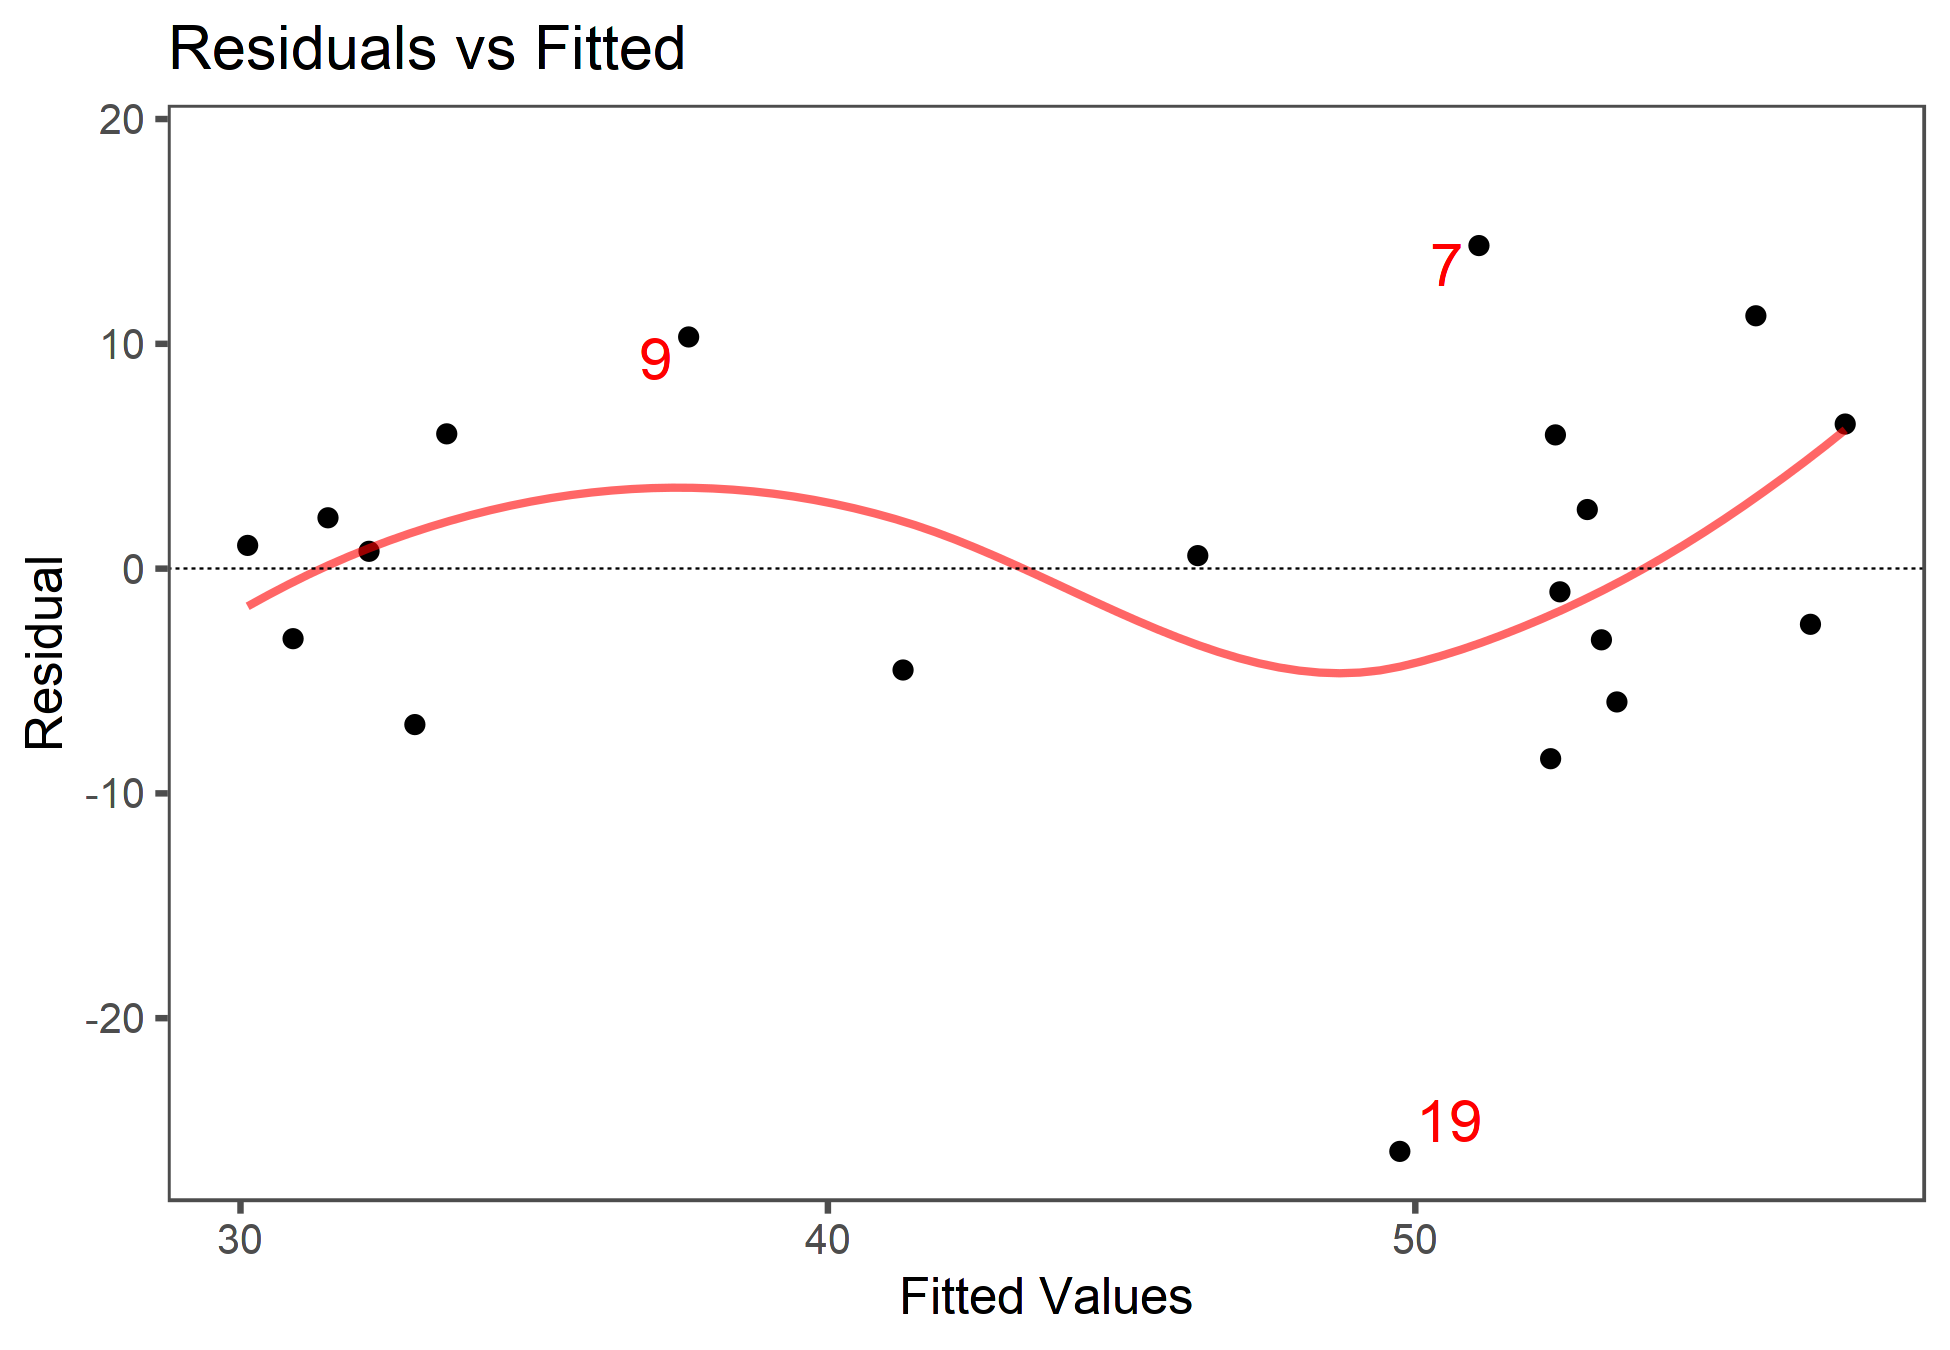
\includegraphics[width=0.3\linewidth]{images/fit-1} 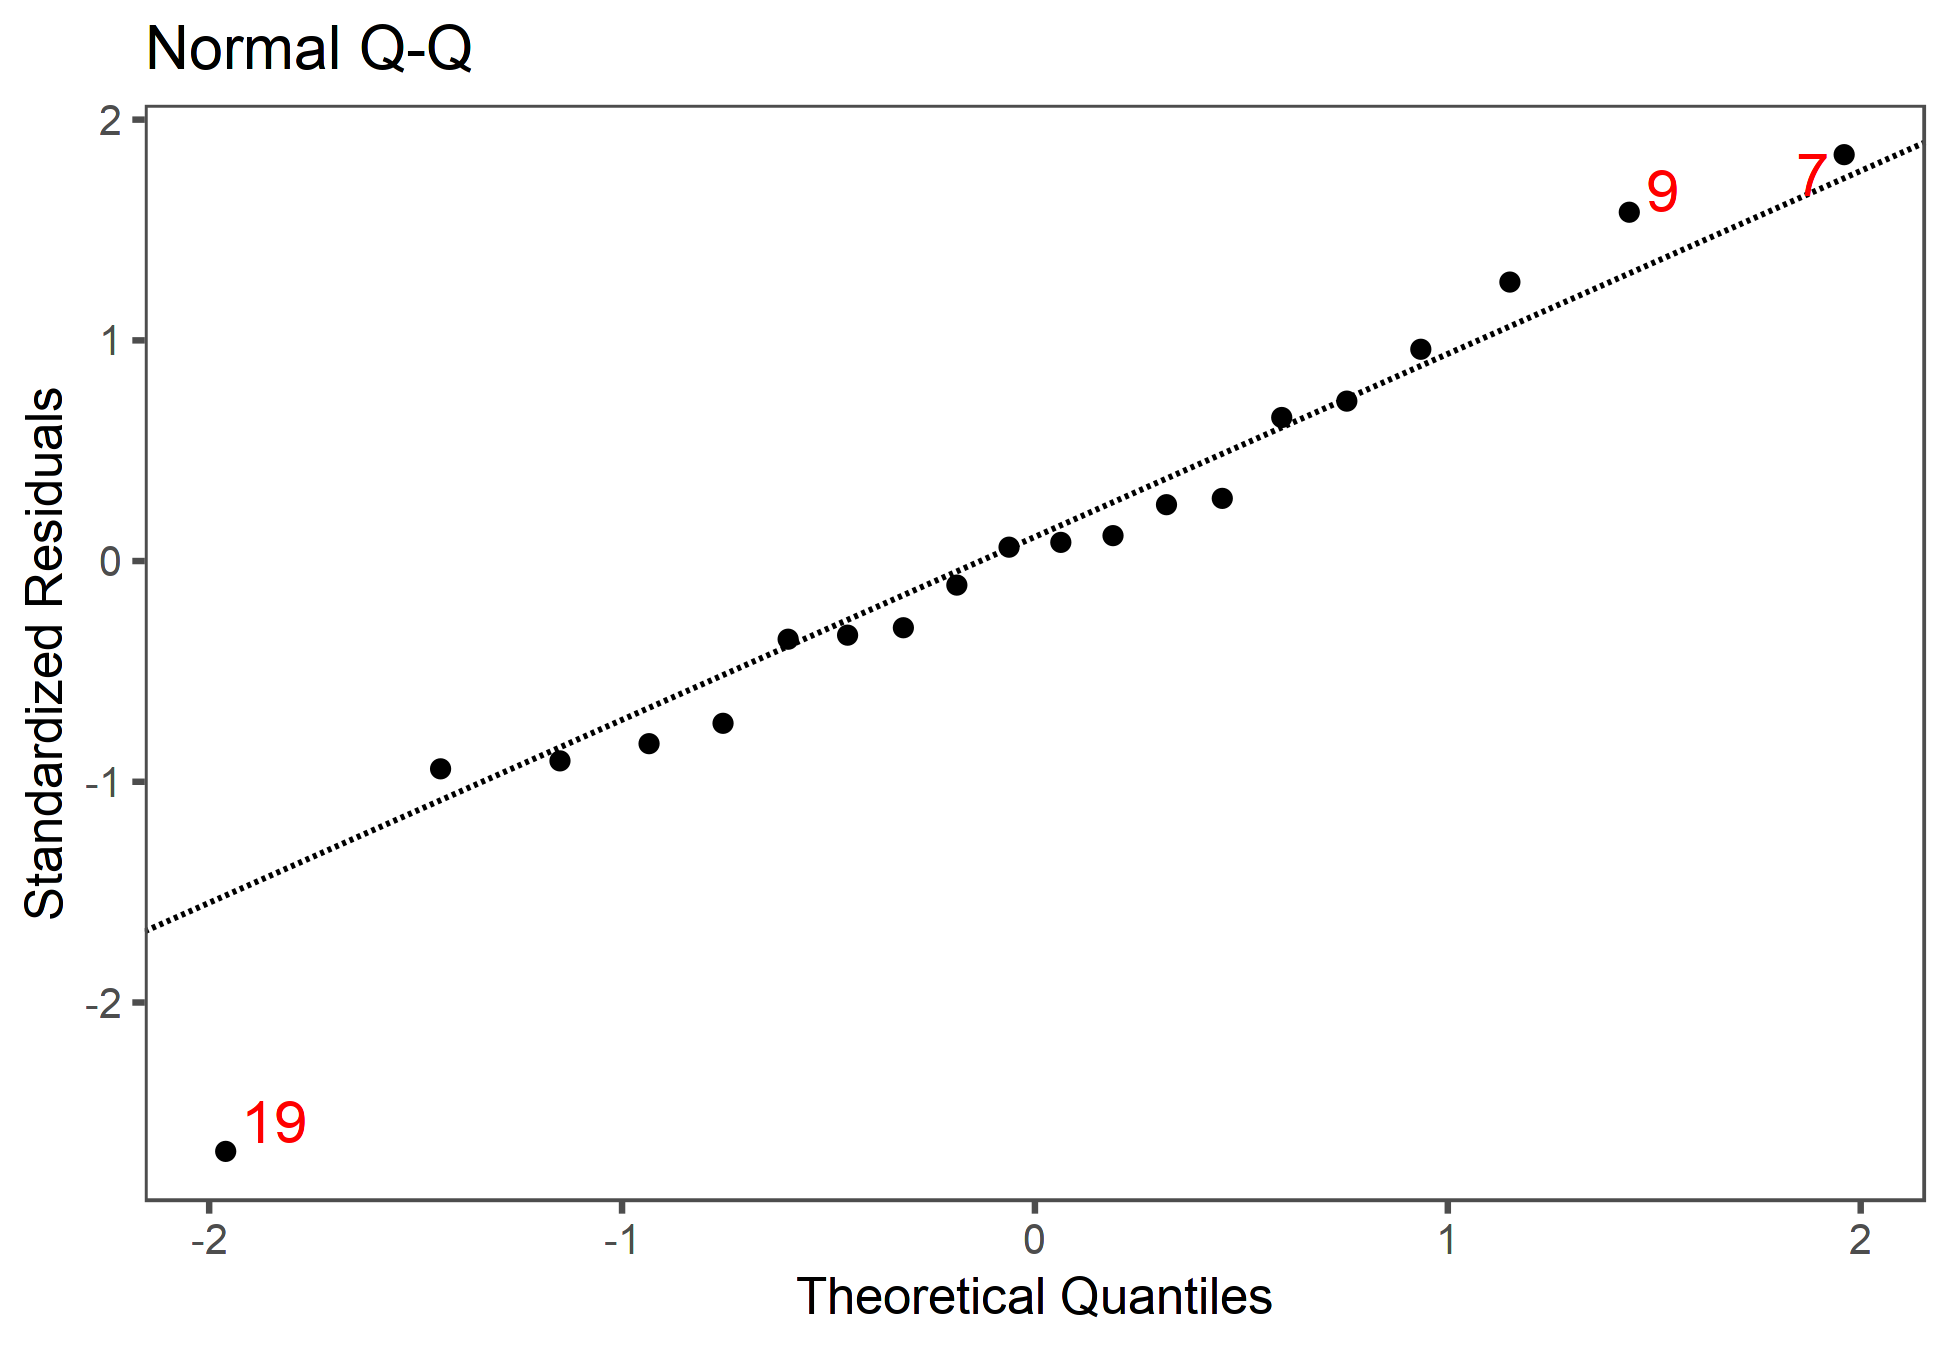
\includegraphics[width=0.3\linewidth]{images/fit-2} 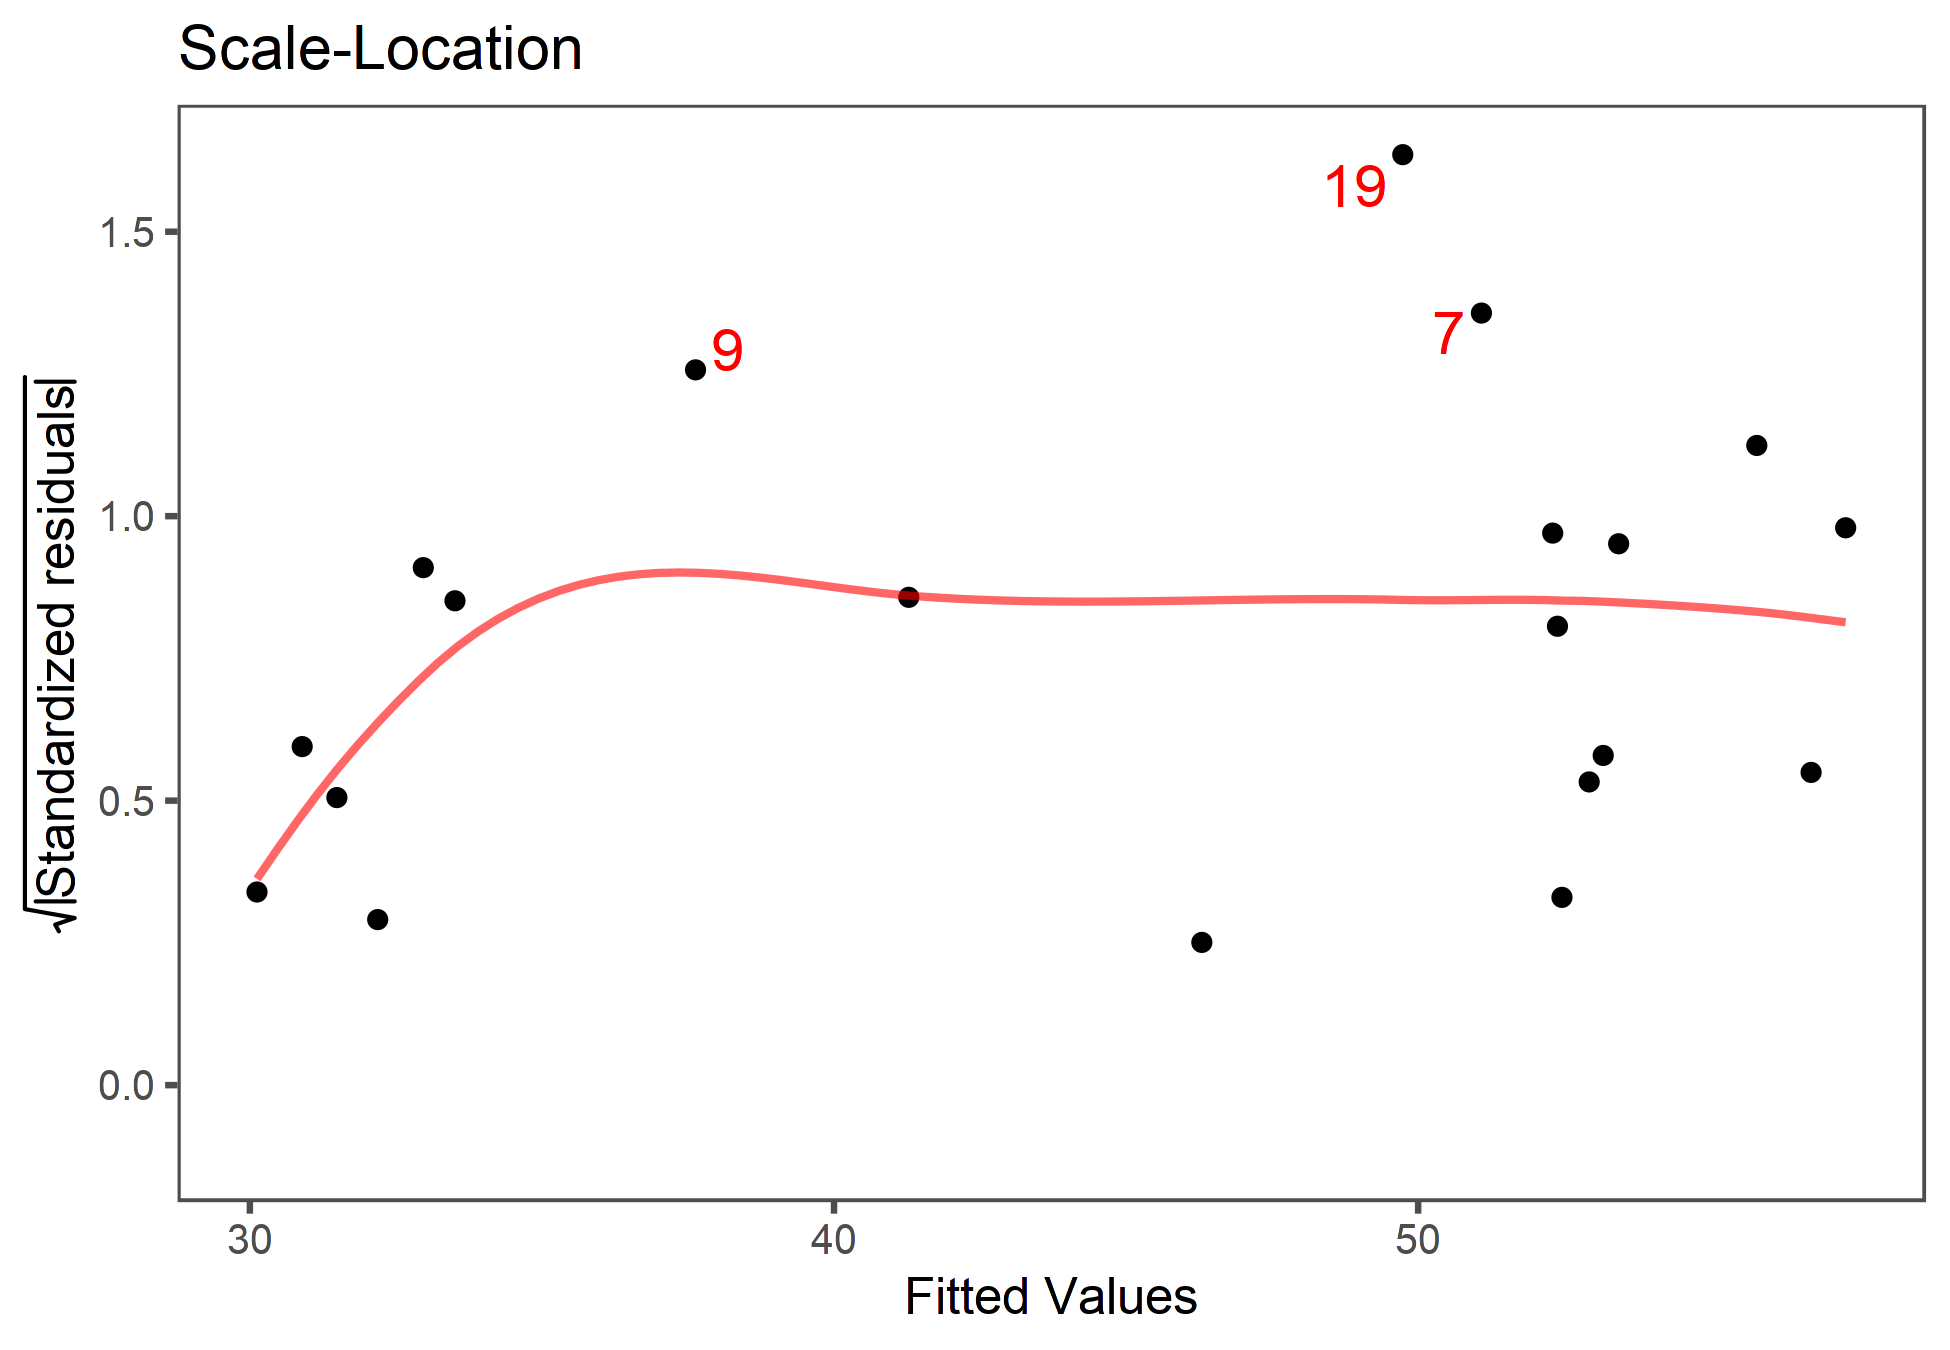
\includegraphics[width=0.3\linewidth]{images/fit-3} 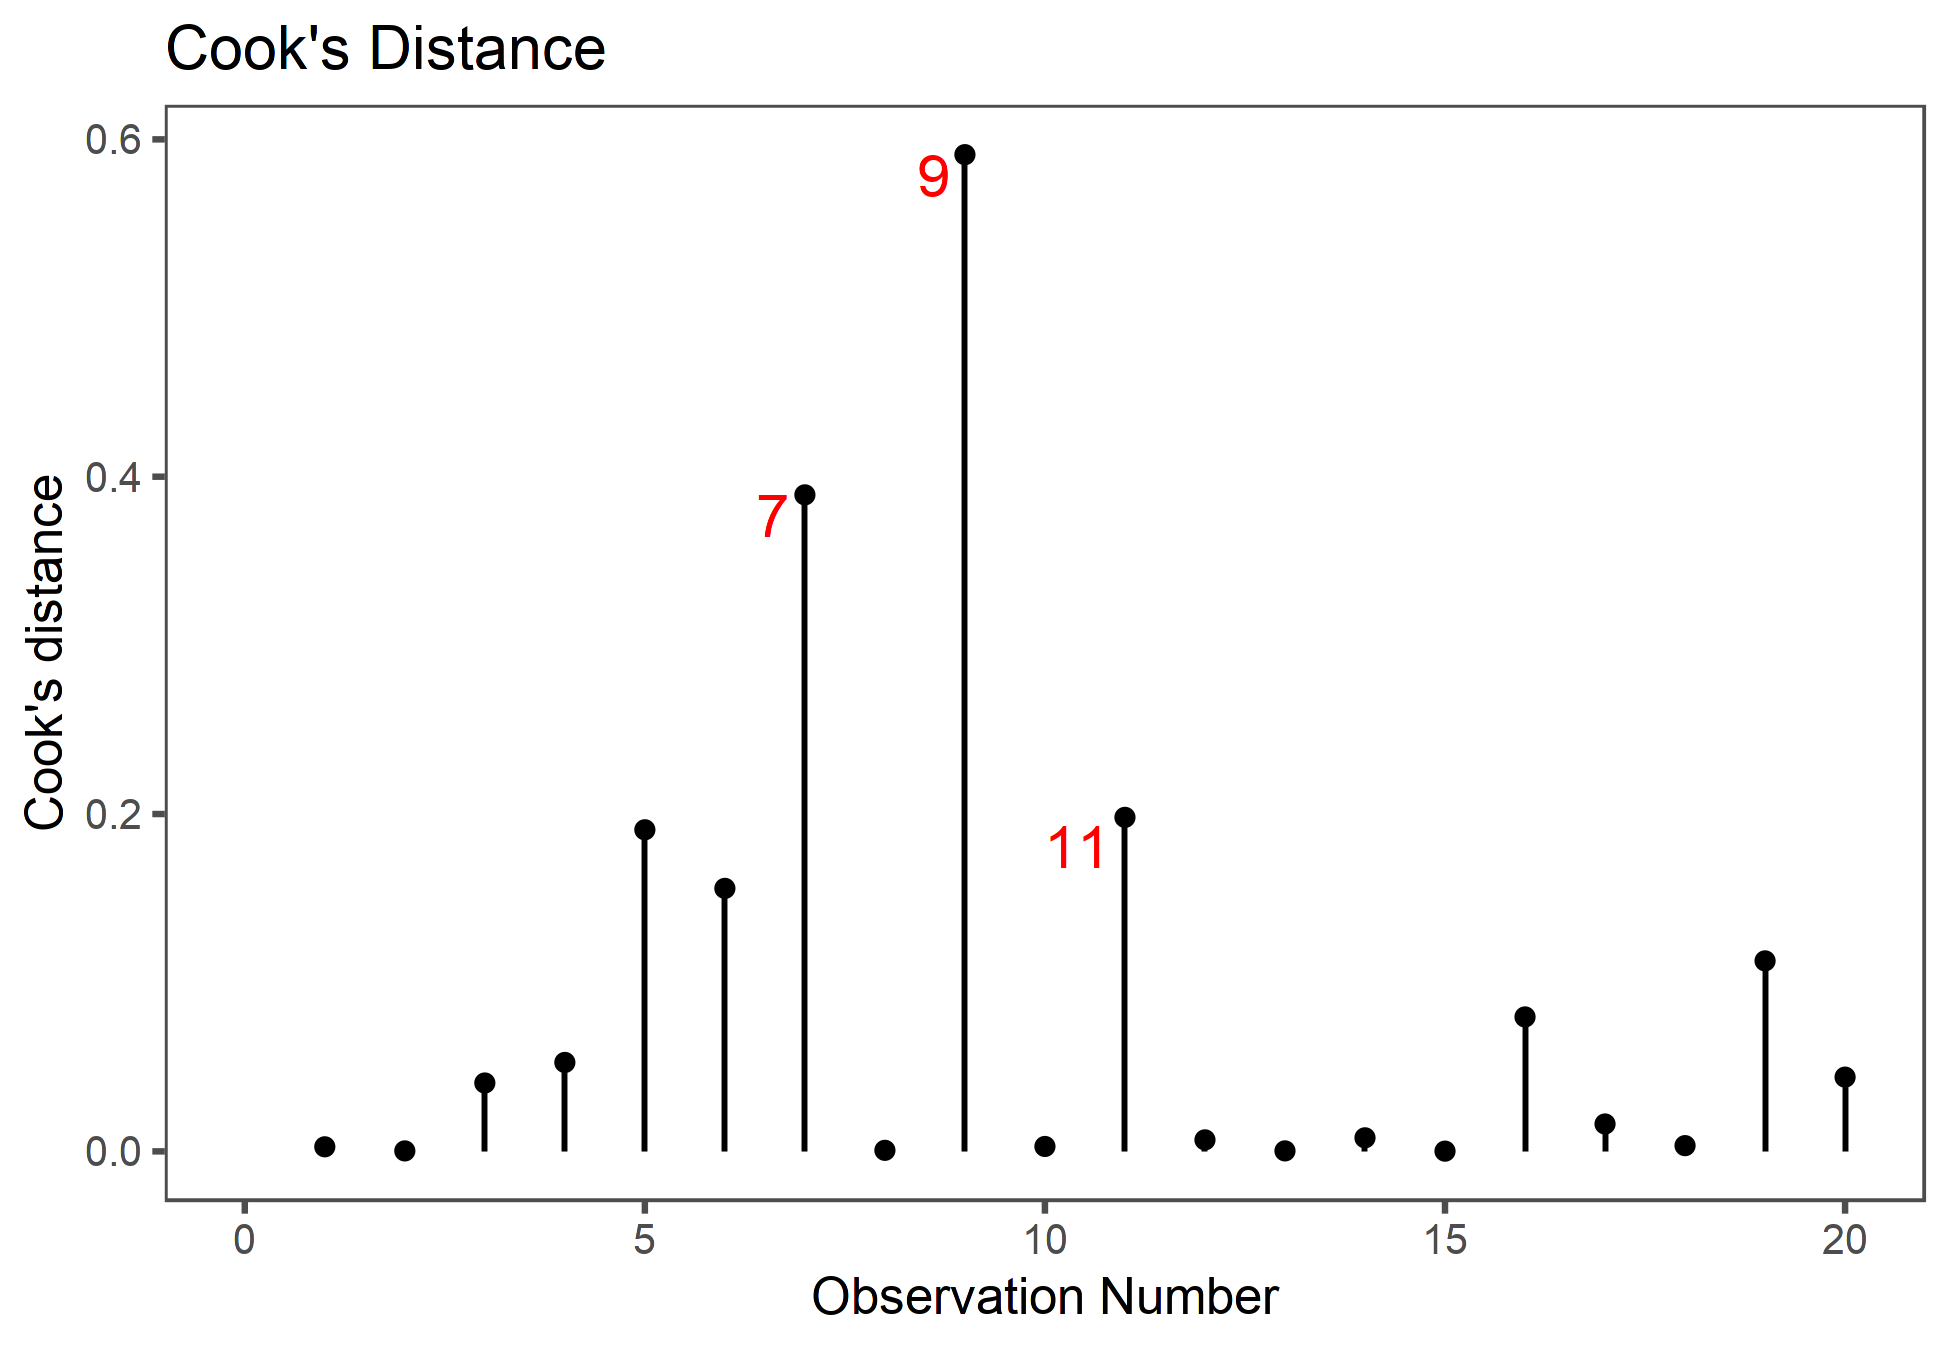
\includegraphics[width=0.3\linewidth]{images/fit-4} 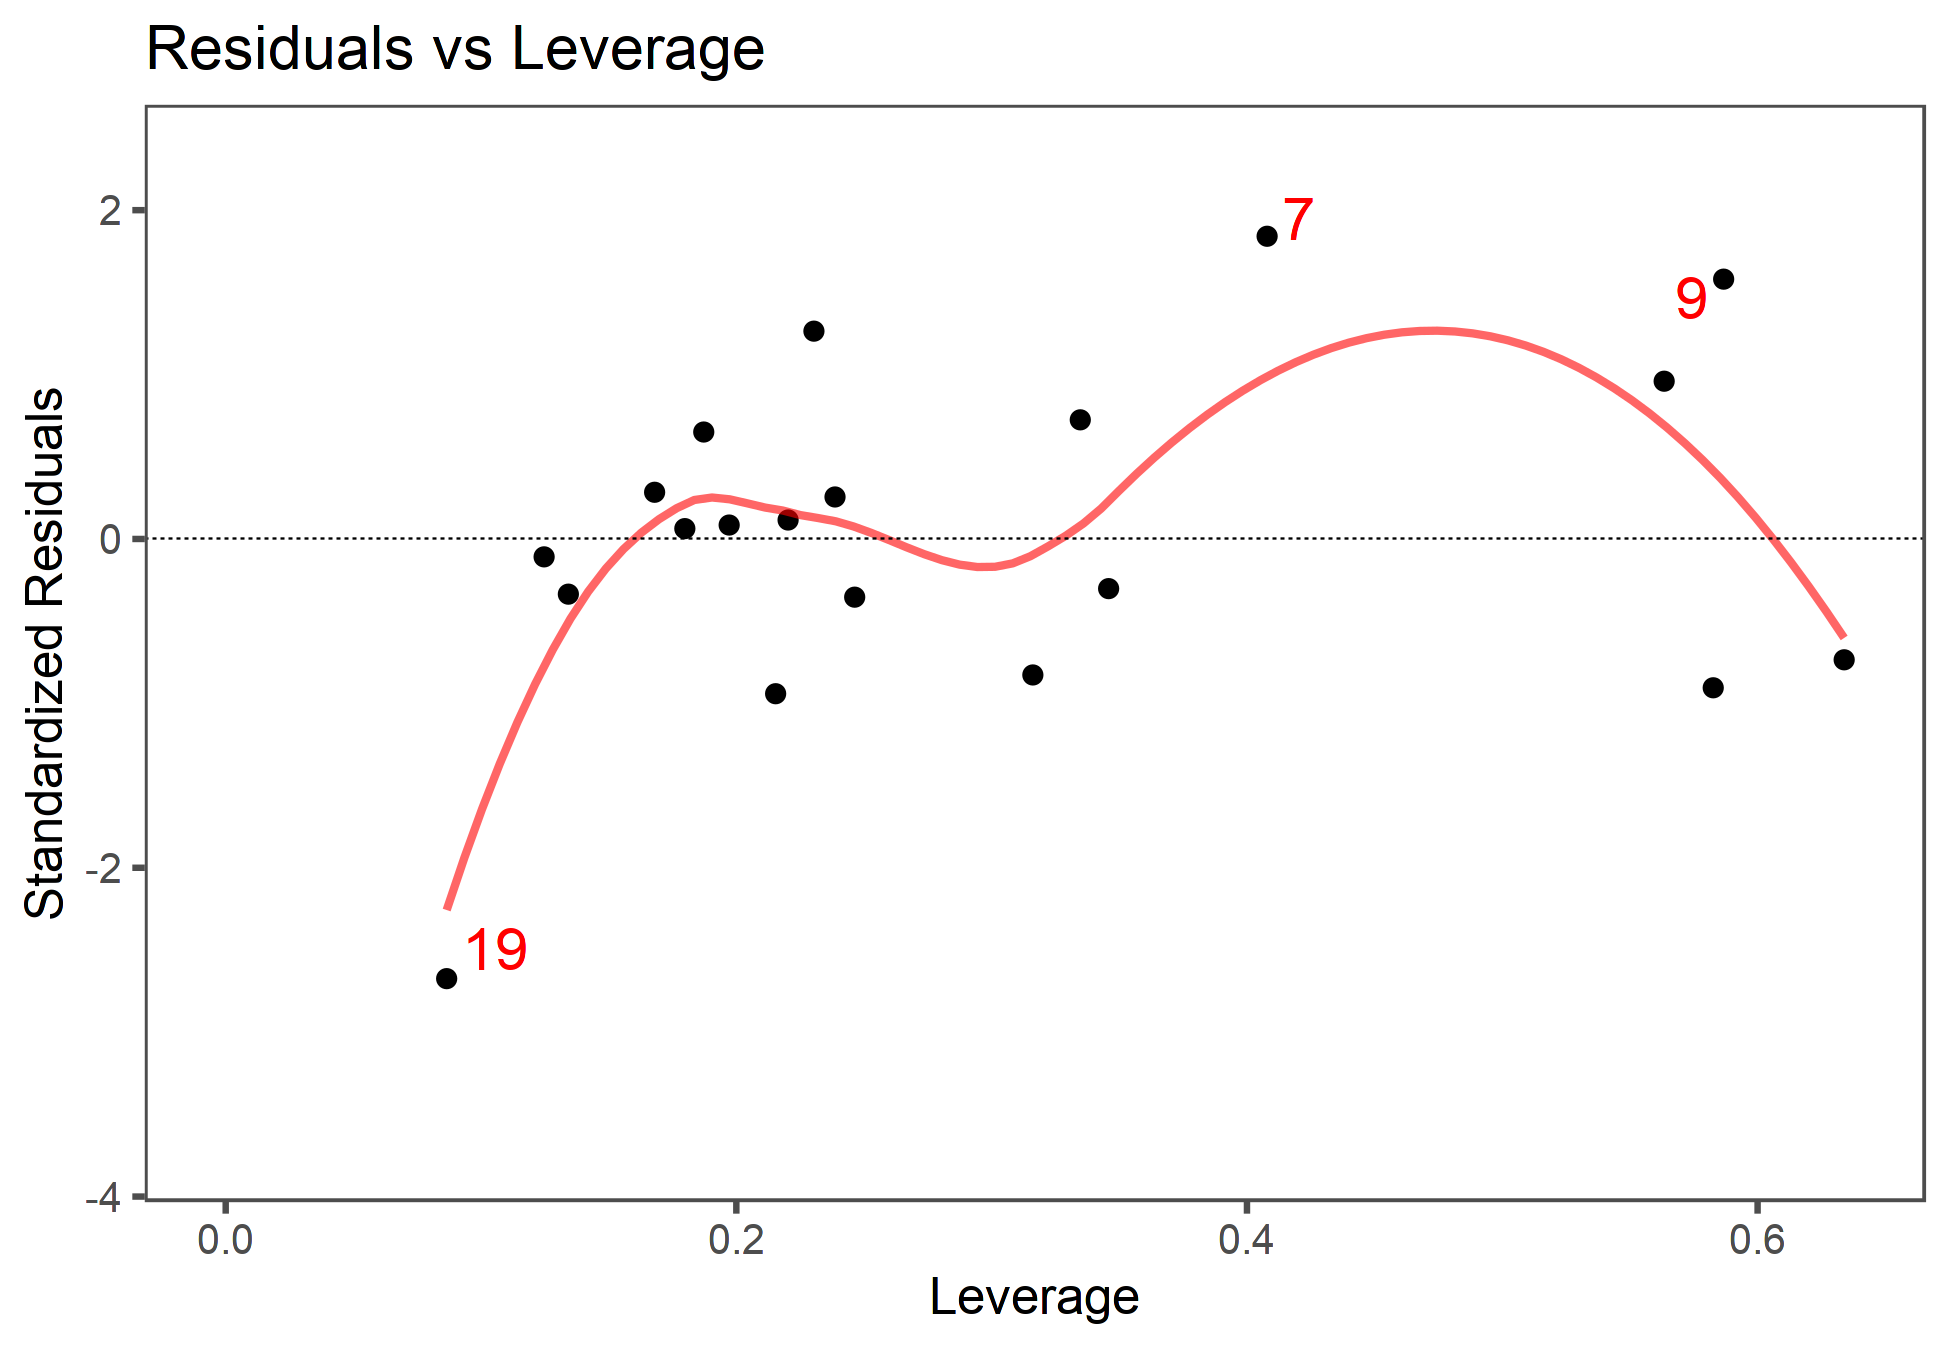
\includegraphics[width=0.3\linewidth]{images/fit-5} 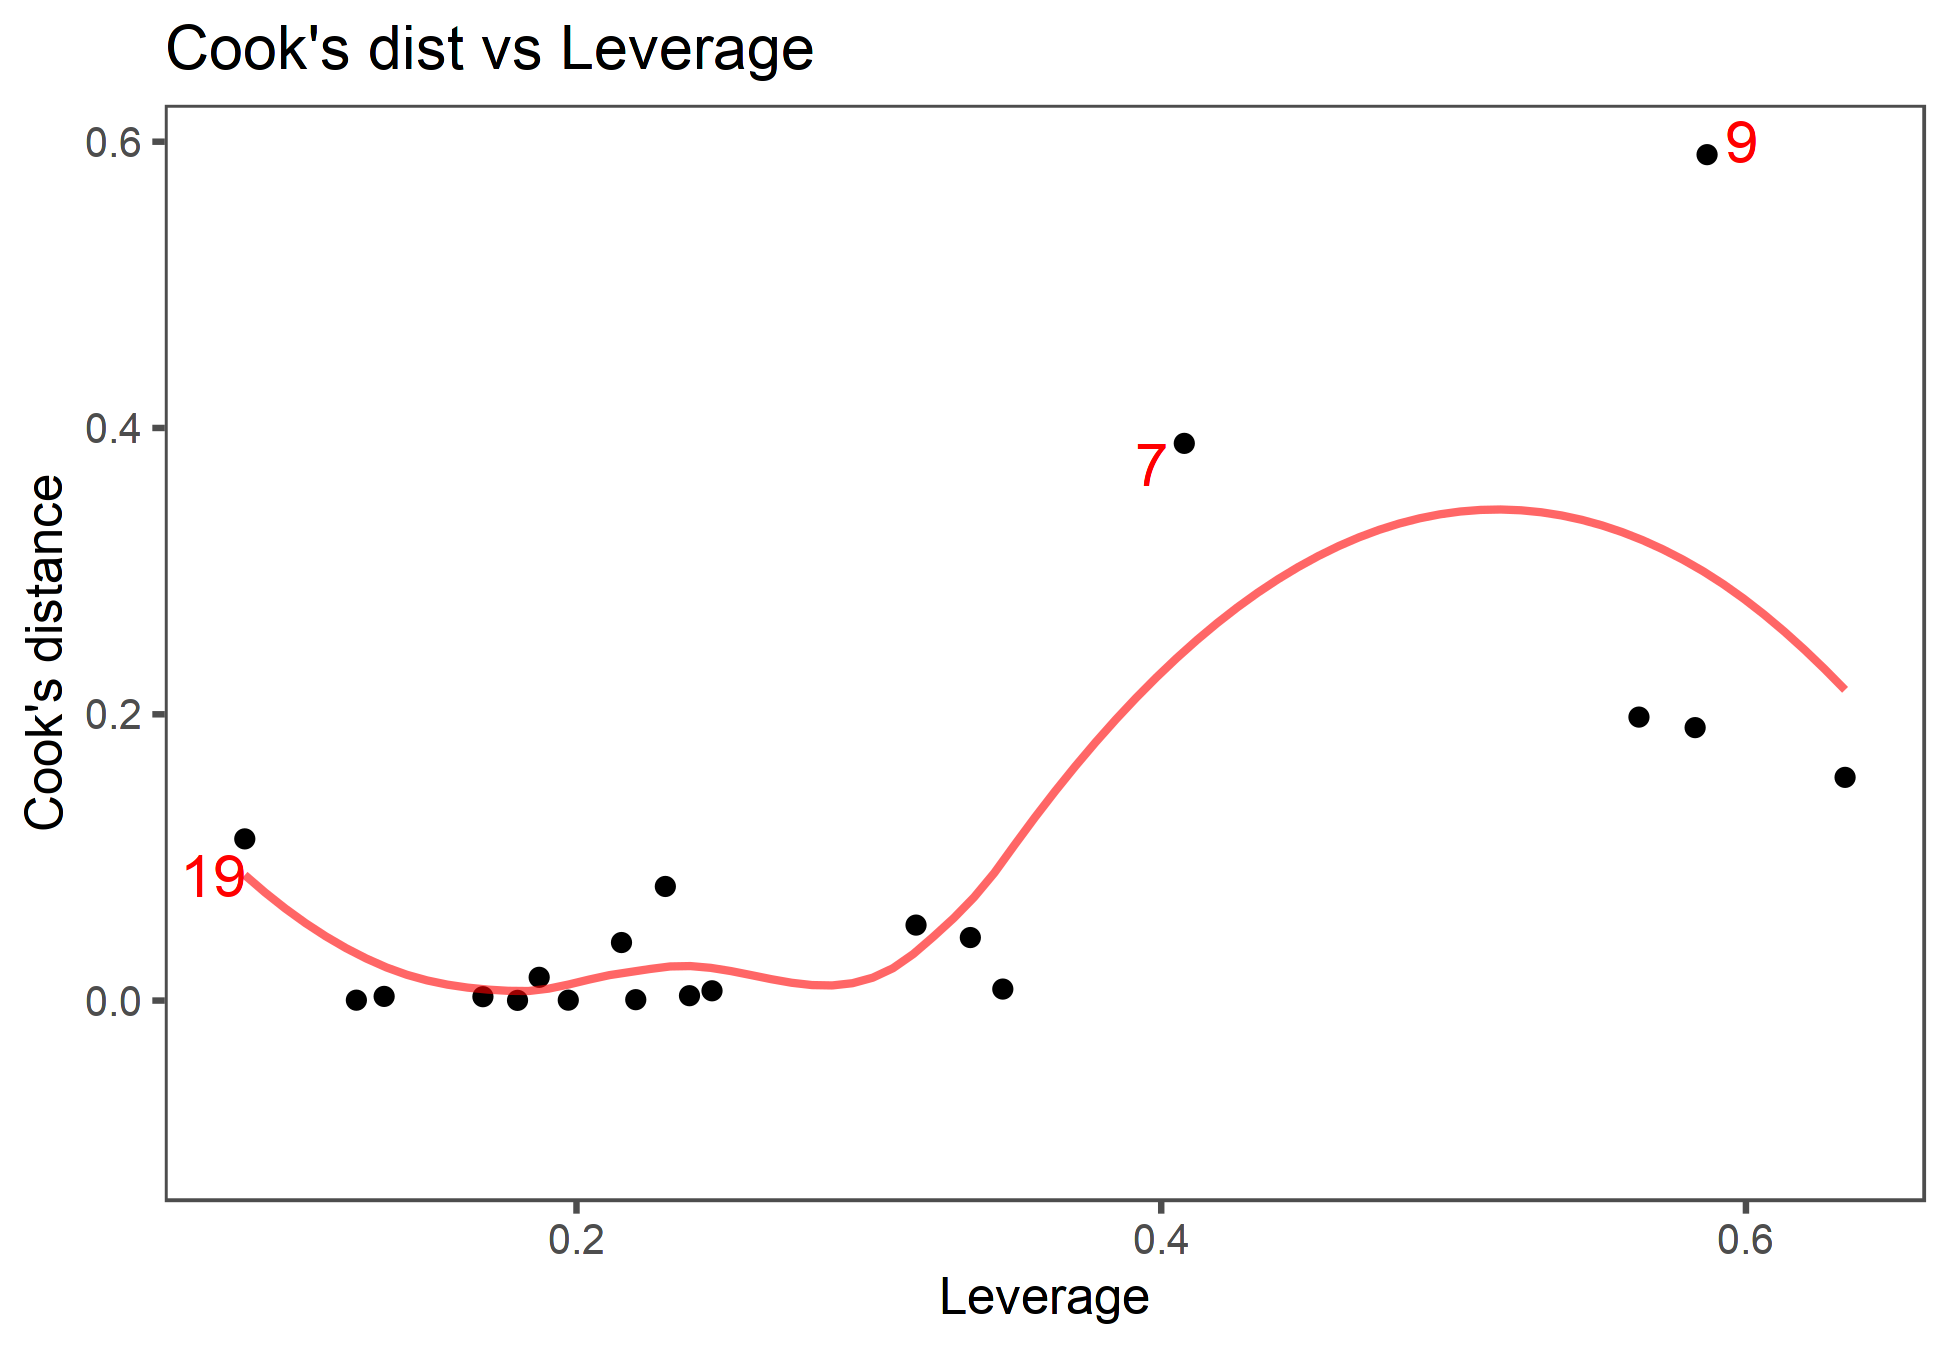
\includegraphics[width=0.3\linewidth]{images/fit-6} 

}

\caption{Modelo com todos os dados}\label{fig:fit}
\end{figure}

Como se pode notar na figura \ref{fig:fit}, os pontos 7 e 19
encontram-se bem afastados da média e foram excluídos do modelo final.

Segundo Hochheim, (\protect\hyperlink{ref-hochheim2005}{2005}, p. 74), o
paradigma da região é um terreno plano e seco, com 15m de frente e 30m
de profundidade.

Uma vez obtido o modelo final saneado, então, foi ajustado outro modelo,
onde adotou-se a centralização das variáveis \texttt{frente} e
\texttt{profundidade}, de acordo com o lote paradigma. Já a variável
\texttt{inclinacao}, por possuir os termos quadrático e cúbico, com vias
de reduzir a multicolinearidade, foi centralizada e escalanoda, de
maneira que a nova variável inclinação tem média zero e desvio-padrão
igual a 1.

Os dois modelos são correspondentes entre si, produzem as mesmas
estimativas, porém apenas o modelo com as variáveis centralizadas e
escalonadas conforme explicitado possui grau I de especificação pela NBR
14.653-02 (\protect\hyperlink{ref-NBR1465302}{2011}), conforme se pode
notar na tabela \ref{tab:fits}.

\begin{figure}[H]

{\centering 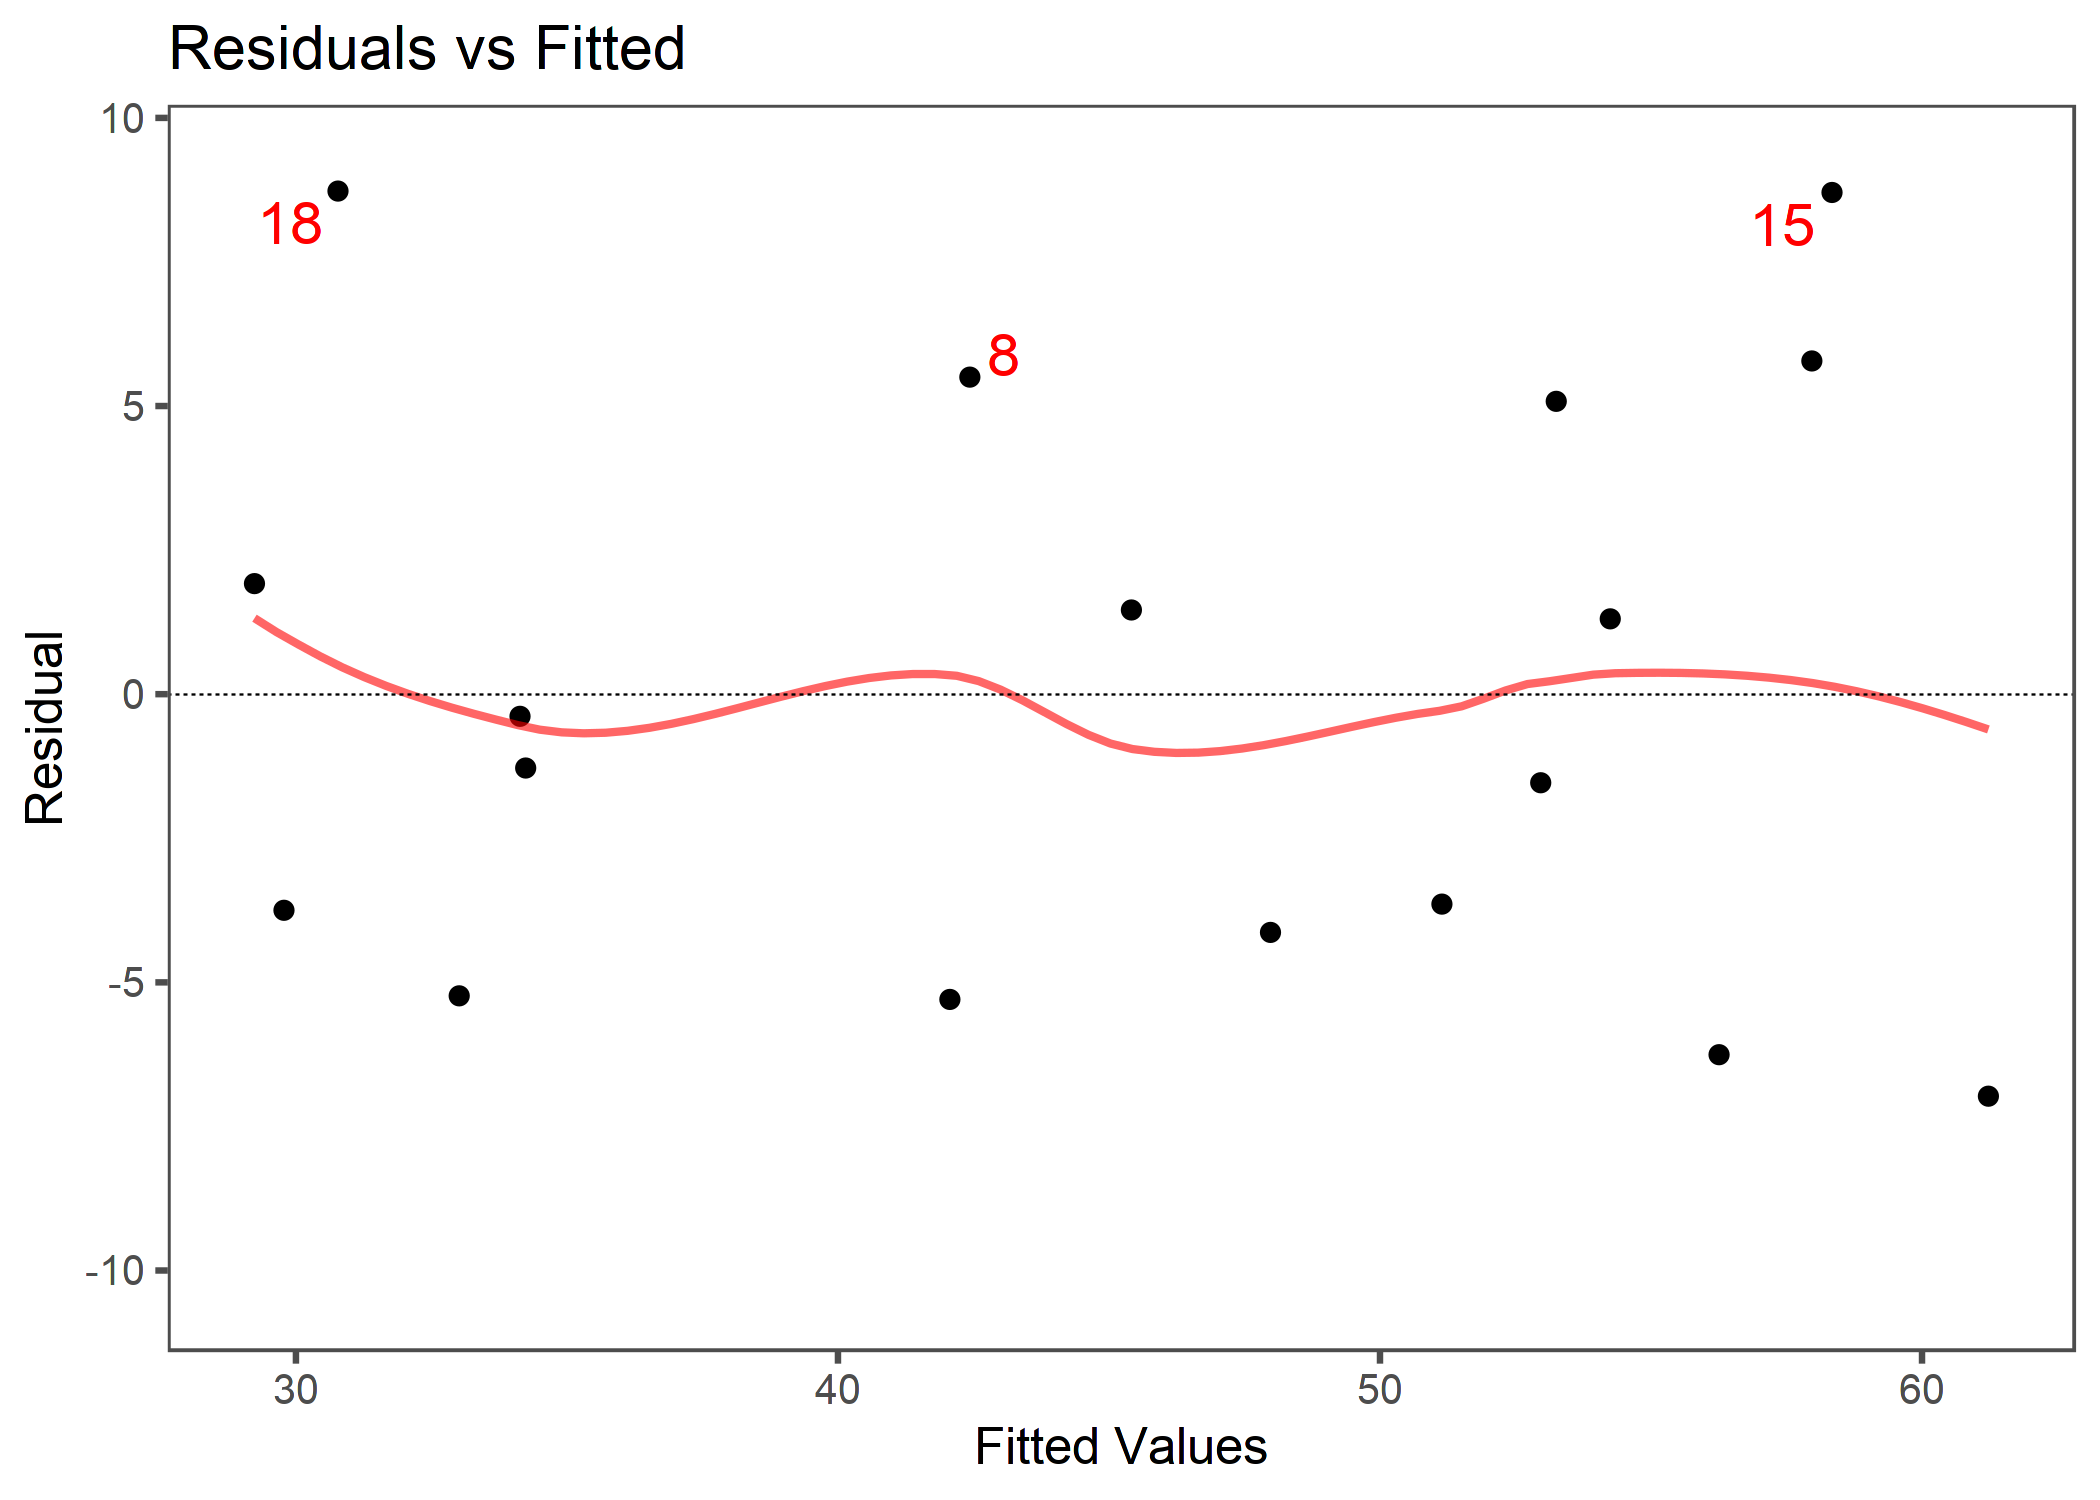
\includegraphics[width=0.3\linewidth]{images/fit1-1} 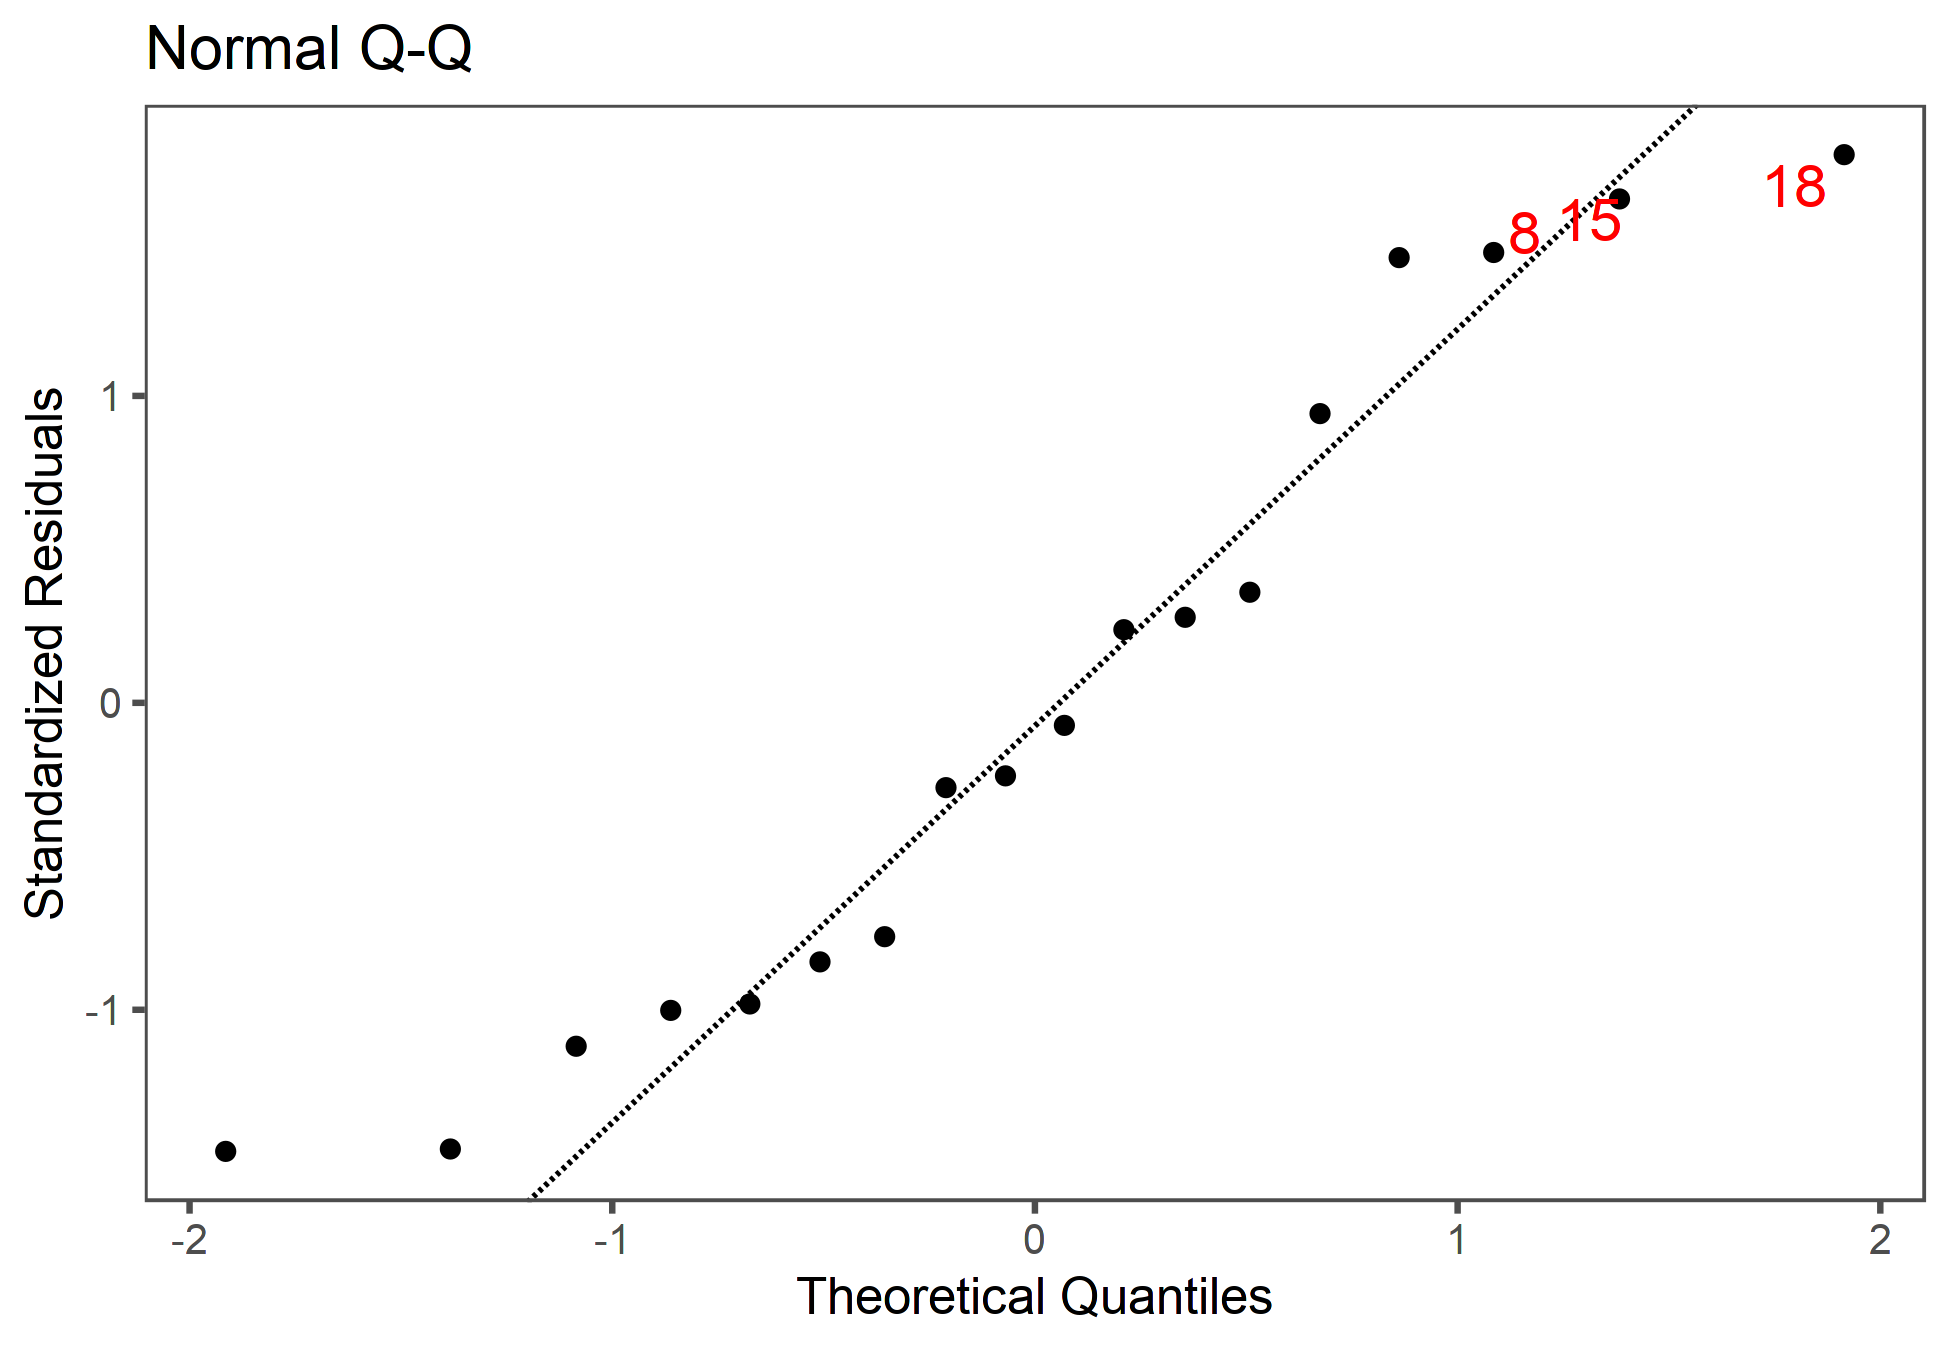
\includegraphics[width=0.3\linewidth]{images/fit1-2} 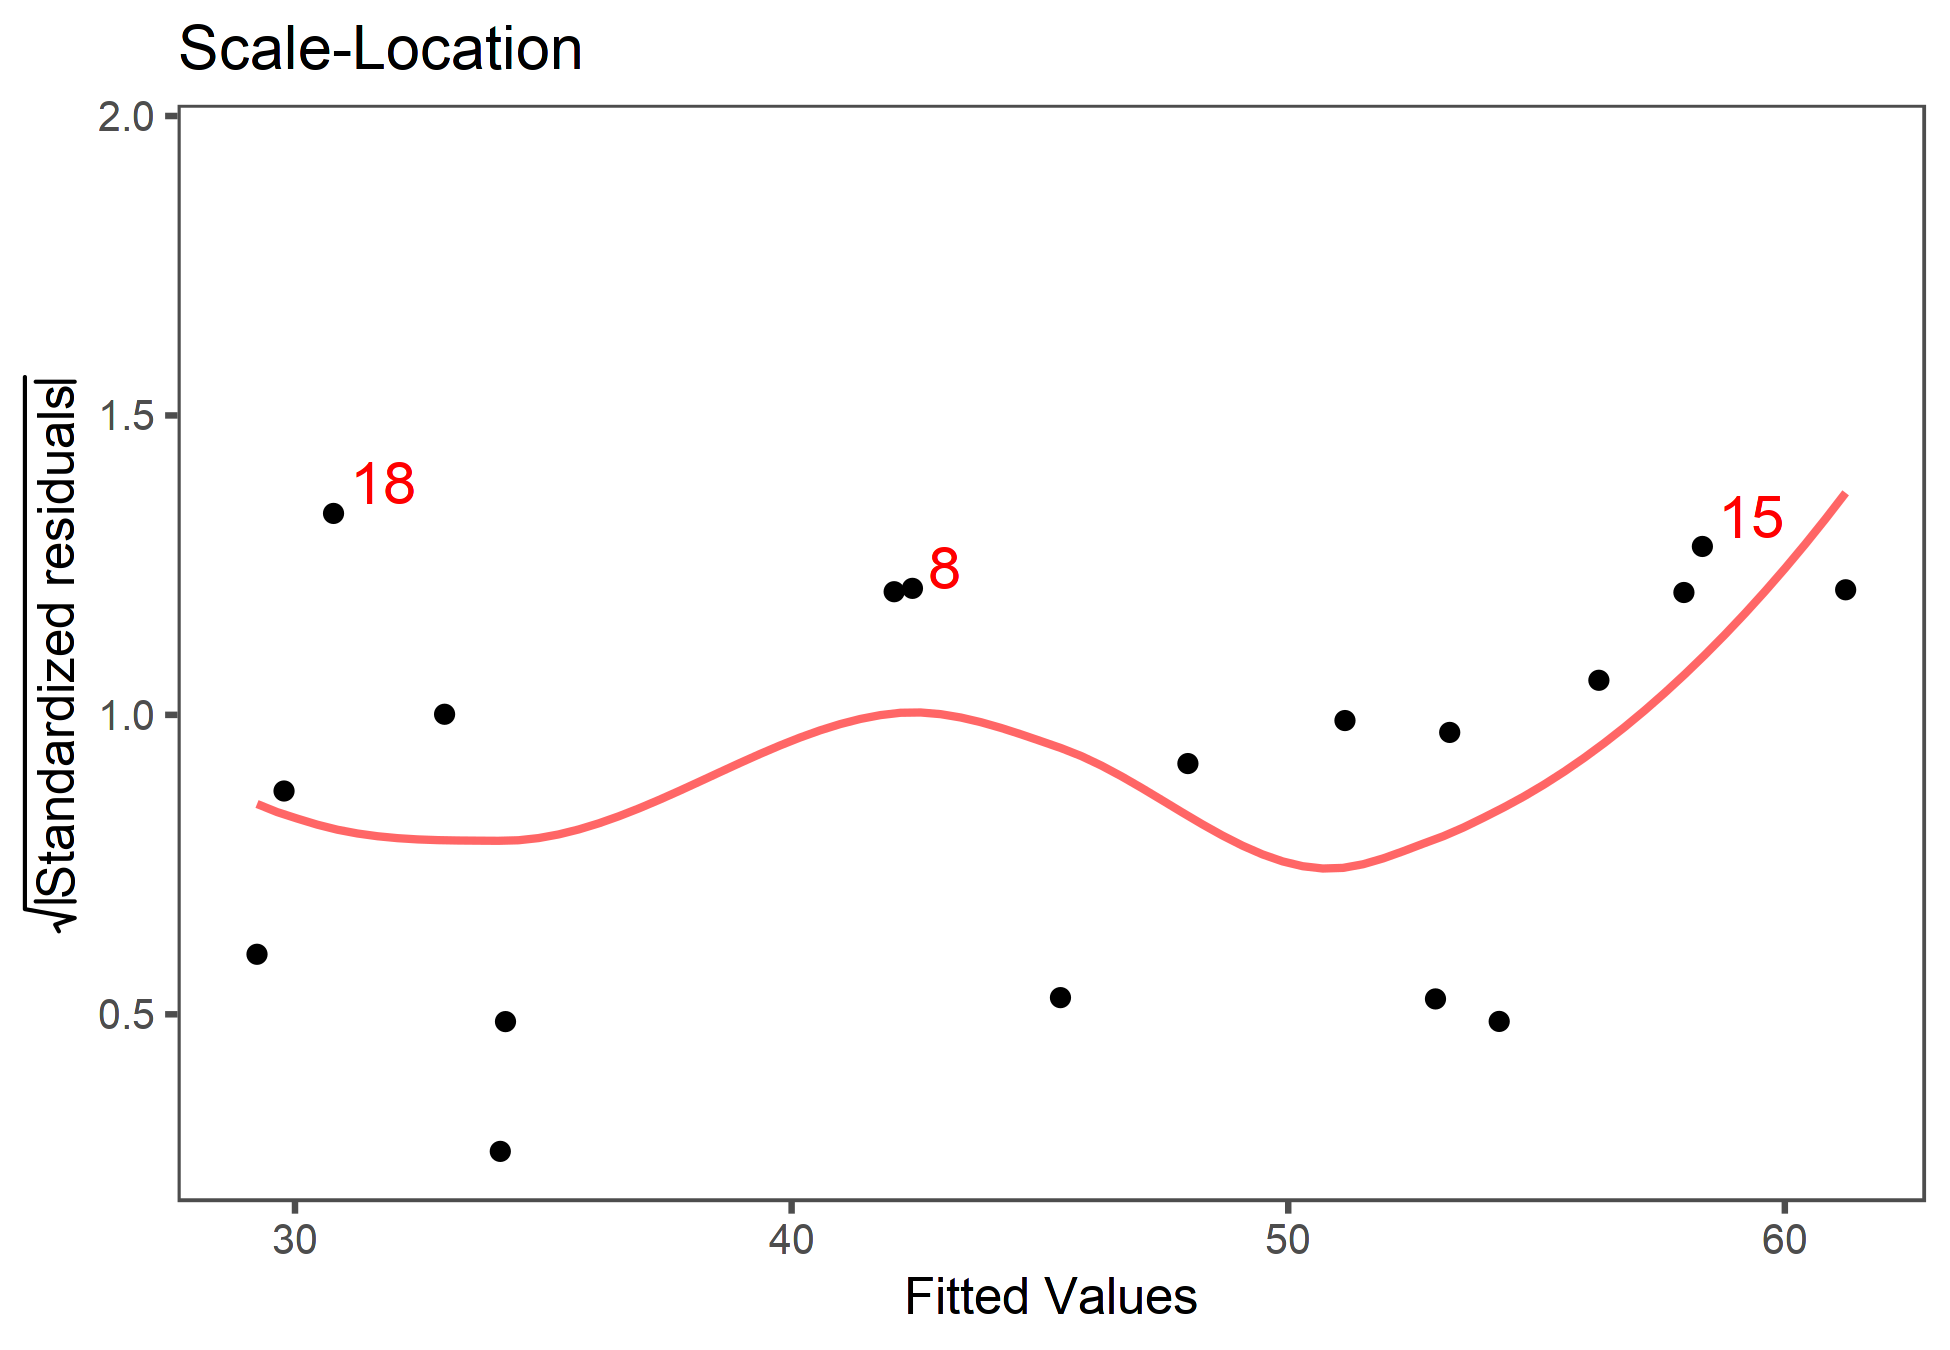
\includegraphics[width=0.3\linewidth]{images/fit1-3} 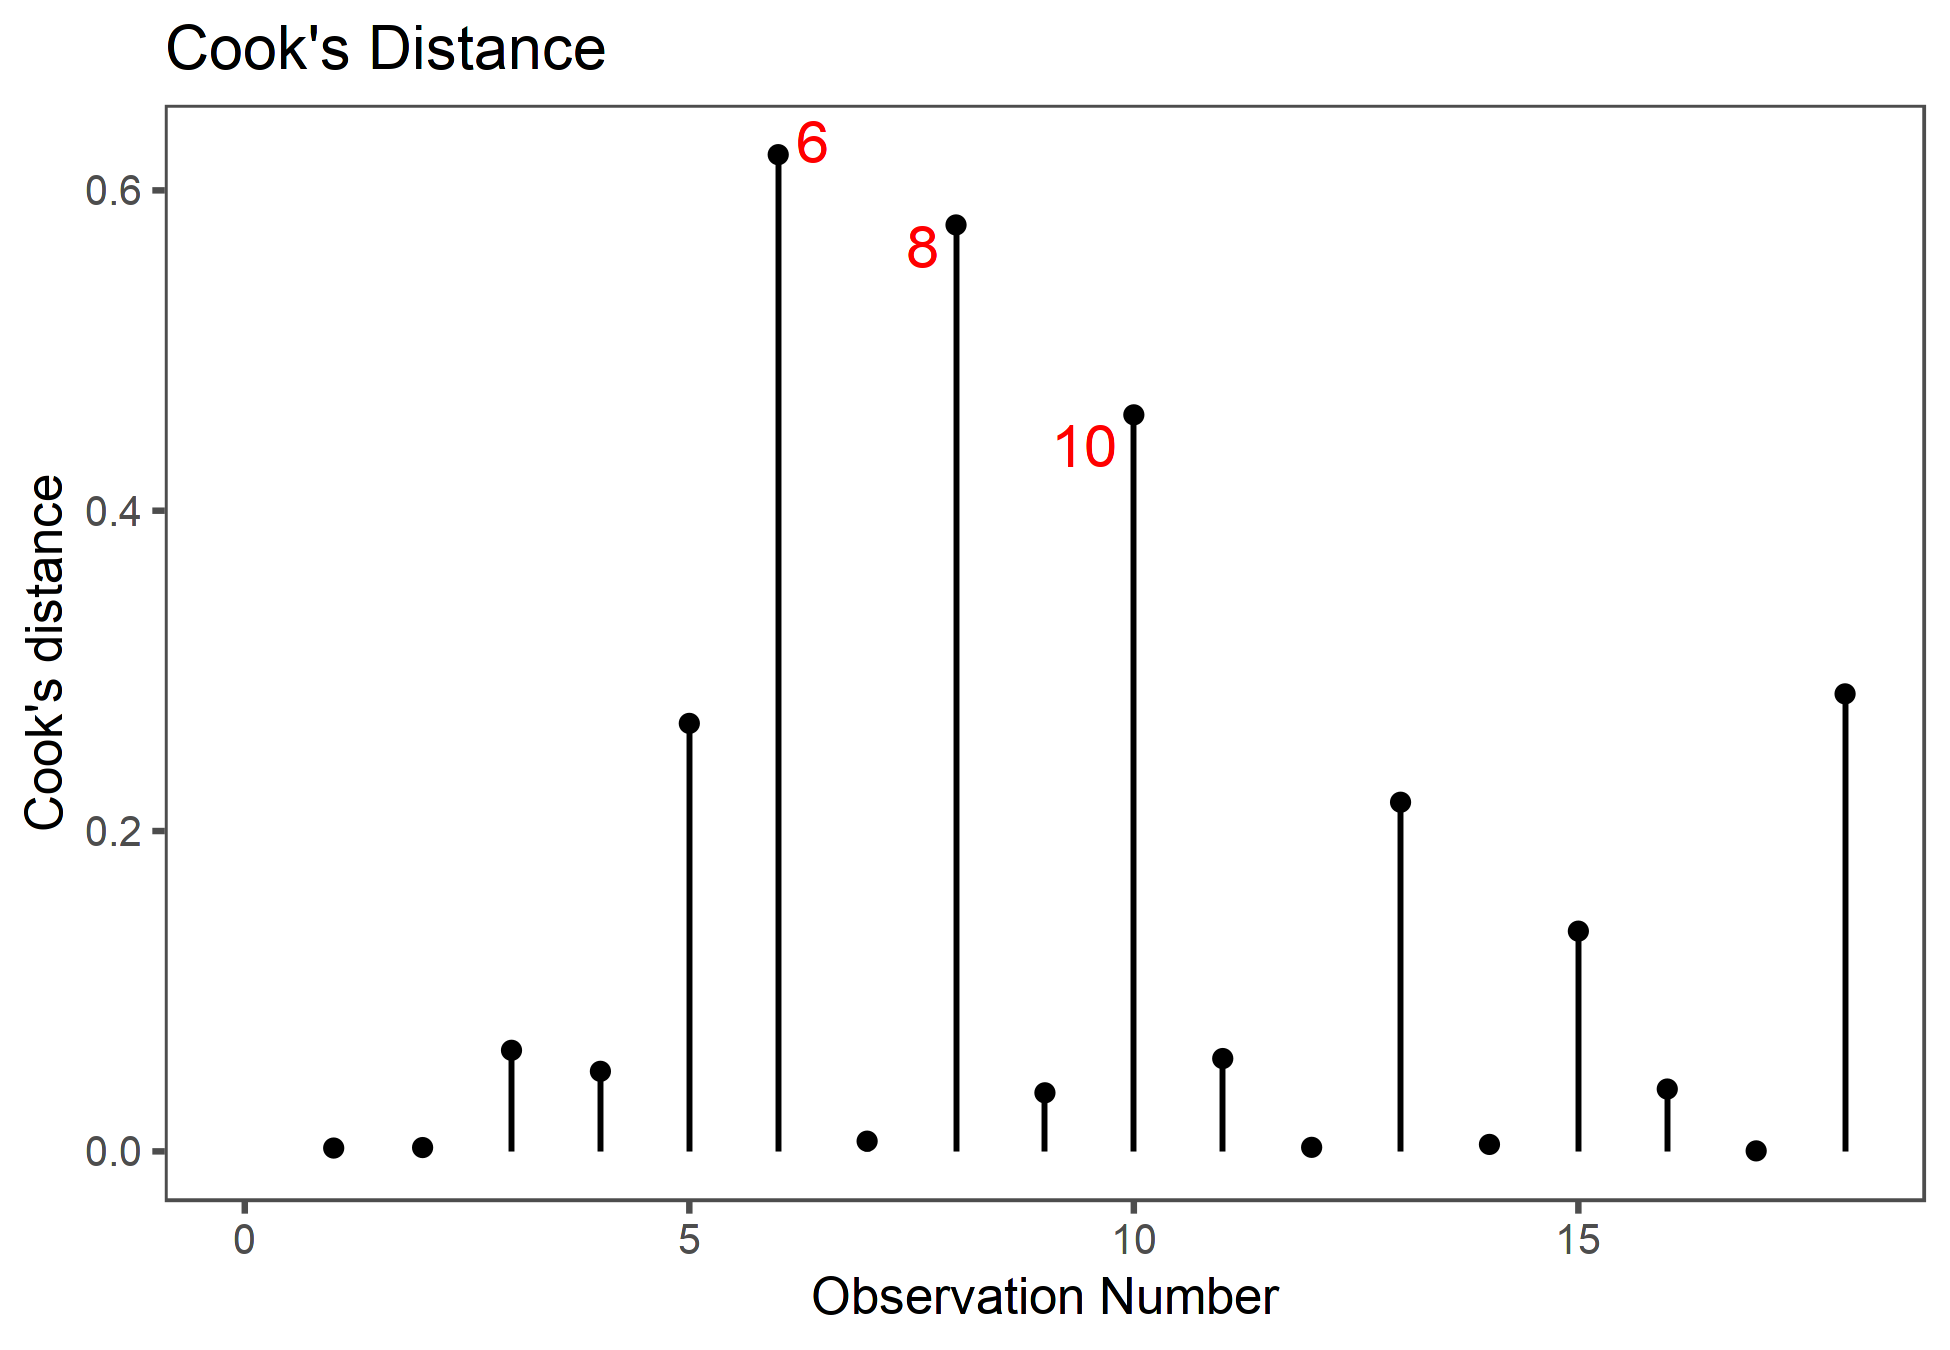
\includegraphics[width=0.3\linewidth]{images/fit1-4} 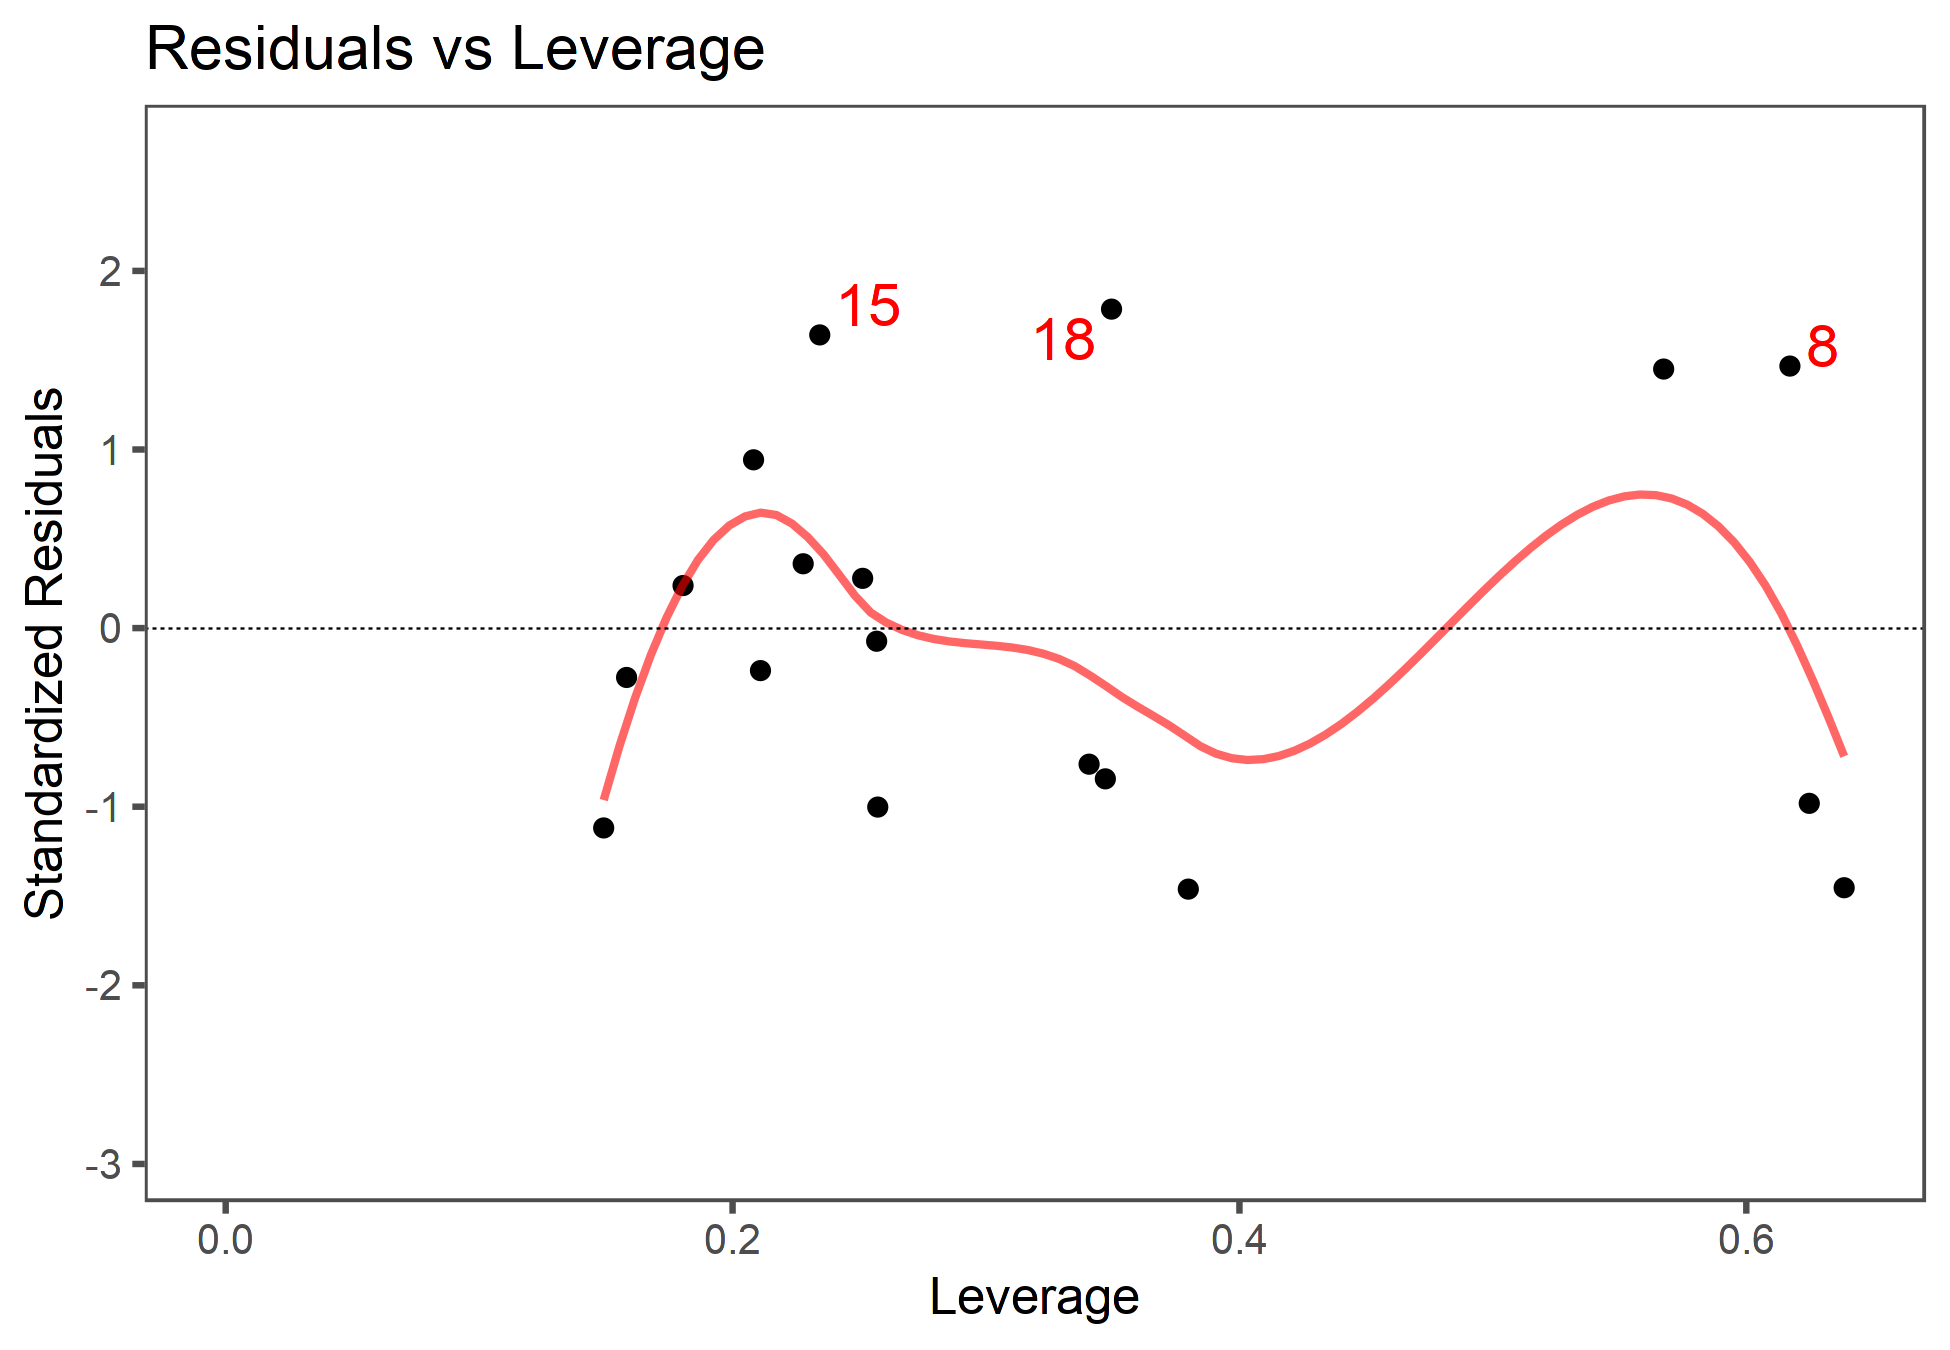
\includegraphics[width=0.3\linewidth]{images/fit1-5} 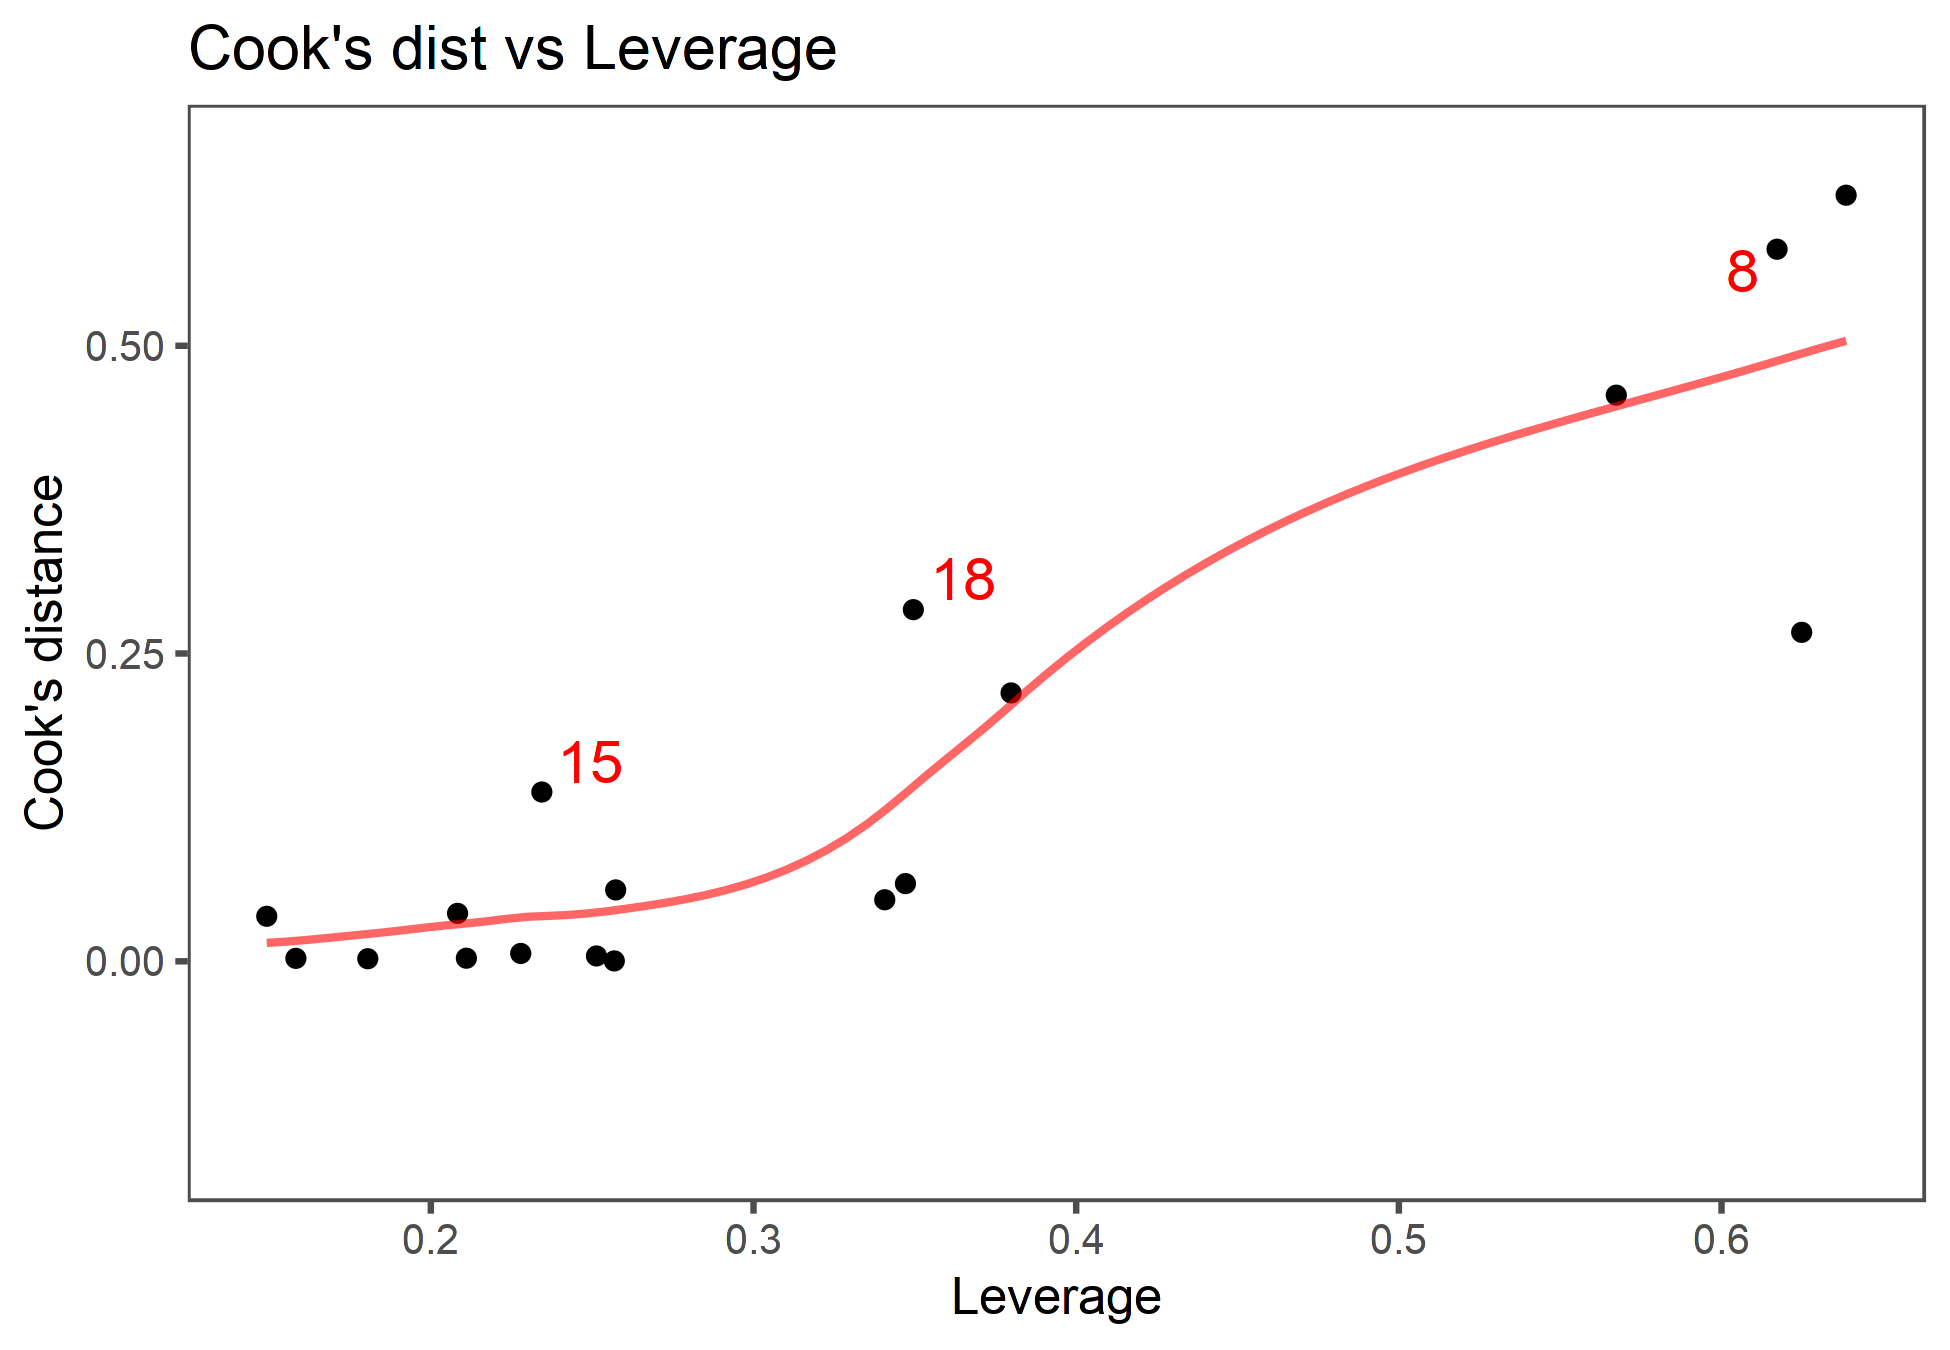
\includegraphics[width=0.3\linewidth]{images/fit1-6} 

}

\caption{Modelo saneado}\label{fig:fit1}
\end{figure}

\begin{table}[!htbp] \centering 
  \caption{Comparacão dos modelos com e sem centralização} 
  \label{tab:fits} 
\begin{tabular}{@{\extracolsep{5pt}}lcc} 
\\[-1.8ex]\hline 
\hline \\[-1.8ex] 
 & \multicolumn{2}{c}{\textit{Dependent variable:}} \\ 
\cline{2-3} 
\\[-1.8ex] & \multicolumn{2}{c}{VU} \\ 
\\[-1.8ex] & (1) & (2)\\ 
\hline \\[-1.8ex] 
 frente & 0,993 & 0,997 \\ 
  & t = 1,954 & t = 1,960 \\ 
  & p = 0,075$^{***}$ & p = 0,074$^{***}$ \\ 
  & & \\ 
 profundidade & $-$0,179 & $-$0,178 \\ 
  & t = $-$1,229 & t = $-$1,220 \\ 
  & p = 0,243$^{*}$ & p = 0,246$^{*}$ \\ 
  & & \\ 
 I(inclinacao$\hat{\mkern6mu}$2) & $-$0,017 & $-$1,617 \\ 
  & t = $-$1,017 & t = $-$1,249 \\ 
  & p = 0,330 & p = 0,236$^{*}$ \\ 
  & & \\ 
 I(inclinacao$\hat{\mkern6mu}$3) & $-$0,001 & $-$0,889 \\ 
  & t = $-$1,390 & t = $-$1,667 \\ 
  & p = 0,190$^{**}$ & p = 0,122$^{**}$ \\ 
  & & \\ 
 pedologiapantanoso & $-$21,201 & $-$21,111 \\ 
  & t = $-$5,689 & t = $-$5,703 \\ 
  & p = 0,0002$^{***}$ & p = 0,0001$^{***}$ \\ 
  & & \\ 
 Constant & 44,813 & 54,265 \\ 
  & t = 4,784 & t = 21,000 \\ 
  & p = 0,0005$^{***}$ & p = 0,000$^{***}$ \\ 
  & & \\ 
\hline \\[-1.8ex] 
Observations & 18 & 18 \\ 
R$^{2}$ & 0,825 & 0,825 \\ 
Adjusted R$^{2}$ & 0,752 & 0,752 \\ 
Residual Std. Error (df = 12) & 6,054 & 6,061 \\ 
F Statistic (df = 5; 12) & 11,323$^{***}$ & 11,291$^{***}$ \\ 
\hline 
\hline \\[-1.8ex] 
\textit{Note:}  & \multicolumn{2}{r}{$^{*}$p$<$0,3; $^{**}$p$<$0,2; $^{***}$p$<$0,1} \\ 
\end{tabular} 
\end{table}

A tabela \ref{tab:tabela} mostra a tabela dos dados amostrais, com o
acréscimo dos valores ajustados.

\begin{longtable}[]{@{}rrlrrlrlrr@{}}
\caption{Dados do modelo com valores ajustados.}\tabularnewline
\toprule
valor & area & tipo & frente & profundidade & topo & inclinacao &
pedologia & VU & yhat\tabularnewline
\midrule
\endfirsthead
\toprule
valor & area & tipo & frente & profundidade & topo & inclinacao &
pedologia & VU & yhat\tabularnewline
\midrule
\endhead
25.000,00 & 450 & venda & 15 & 30 & plano & -0,11 & seco & 55,56 &
54,25\tabularnewline
30.000,00 & 525 & oferta & 15 & 35 & aclive & 0,45 & seco & 51,43 &
52,97\tabularnewline
28.500,00 & 650 & venda & 13 & 50 & declive & -0,99 & seco & 43,85 &
47,98\tabularnewline
29.500,00 & 1.020 & oferta & 17 & 60 & plano & -0,11 & pantanoso & 26,03
& 29,78\tabularnewline
19.000,00 & 360 & oferta & 12 & 30 & declive & -1,77 & seco & 47,50 &
51,14\tabularnewline
44.122,04 & 1.200 & venda & 20 & 60 & aclive & 1,89 & seco & 36,77 &
42,06\tabularnewline
40.000,00 & 550 & oferta & 10 & 55 & declive & -1,22 & seco & 65,45 &
44,03\tabularnewline
18.000,00 & 520 & oferta & 13 & 40 & declive & -0,33 & pantanoso & 31,15
& 29,23\tabularnewline
21.570,77 & 450 & venda & 15 & 30 & aclive & 1,89 & seco & 47,94 &
42,43\tabularnewline
23.000,00 & 414 & oferta & 18 & 30 & aclive & 0,67 & seco & 50,00 &
56,26\tabularnewline
25.500,00 & 400 & venda & 20 & 35 & declive & -1,66 & seco & 63,75 &
57,97\tabularnewline
12.500,00 & 450 & venda & 15 & 30 & declive & -0,33 & pantanoso & 27,78
& 33,01\tabularnewline
19.609,79 & 595 & venda & 17 & 35 & plano & -0,11 & pantanoso & 32,96 &
34,24\tabularnewline
30.500,00 & 506 & oferta & 22 & 30 & plano & -0,11 & seco & 54,25 &
61,22\tabularnewline
25.000,00 & 480 & oferta & 12 & 40 & aclive & 1,23 & seco & 46,88 &
45,41\tabularnewline
29.500,00 & 440 & venda & 20 & 35 & plano & -0,11 & seco & 67,05 &
58,34\tabularnewline
24.500,00 & 420 & venda & 14 & 30 & plano & -0,11 & seco & 58,33 &
53,25\tabularnewline
18.000,00 & 480 & oferta & 16 & 30 & plano & -0,11 & pantanoso & 33,75 &
34,13\tabularnewline
12.500,00 & 525 & venda & 15 & 35 & aclive & 1,00 & seco & 23,81 &
50,84\tabularnewline
32.000,00 & 810 & venda & 18 & 60 & plano & -0,11 & pantanoso & 39,51 &
30,78\tabularnewline
\bottomrule
\end{longtable}

A figura \ref{fig:pplot} mostra o gráfico do poder de predição do
modelo.

\begin{figure}[H]

{\centering 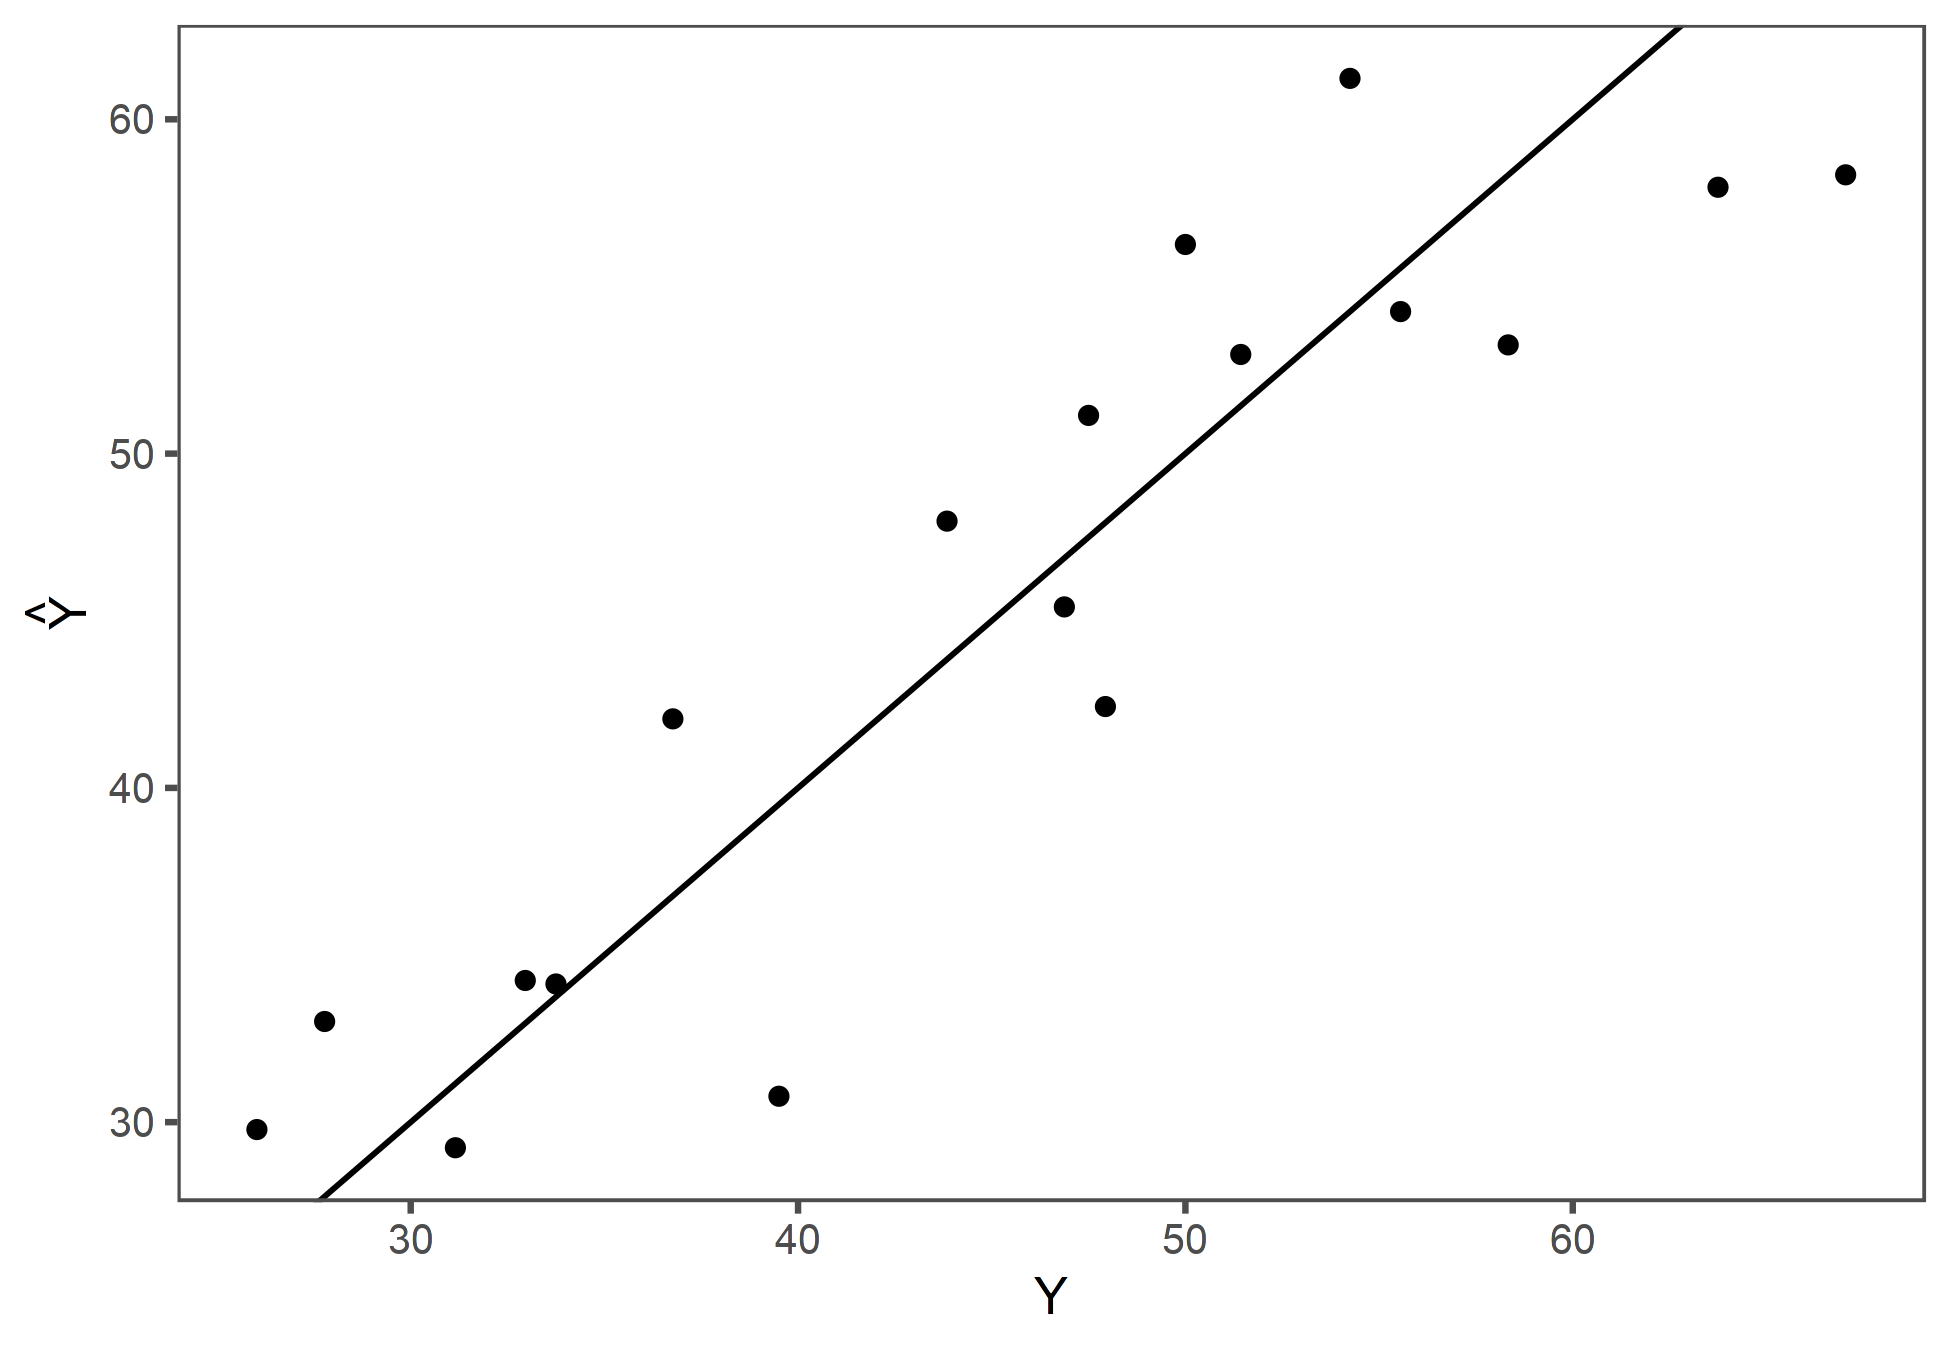
\includegraphics[width=0.7\linewidth]{images/pplot-1} 

}

\caption{Poder de predição do modelo.}\label{fig:pplot}
\end{figure}

\hypertarget{coerencia-do-modelo}{%
\subsection{Coerência do modelo}\label{coerencia-do-modelo}}

O modelo é coerente, conforme pode-se notar nas estimativas abaixo:

Segundo o modelo, o lote paradigma vale R\$54,25/\(m^2\), o que é muito
próximo do intercepto do modelo final (R\$ 54,27/\(m^2\)). Apenas para
efeito de comparação, o mesmo lote paradigma avaliado de acordo com o
modelo com os dados originais vale 54,33/\(m^2\).

Um lote com as mesmas características do lote paradigma, porém com 5m a
mais de frente, segundo o modelo, vale R\$59,23/\(m^2\). No modelo
original, vale 59,30/\(m^2\).

Um lote com as mesmas características do lote paradigma, porém com 45m
de profundidade, segundo o modelo, vale R\$51,57/\(m^2\). No modelo
original, vale 51,64/\(m^2\).

Um lote com as mesmas características do lote paradigma, porém com 20m
de frente e 45m de profundidade, segundo o modelo, vale
R\$56,56/\(m^2\). No modelo original, vale 56,61/\(m^2\).

Um lote com as mesmas características do lote paradigma, porém com
declive de 10\%, segundo o modelo, vale R\$53,47/\(m^2\). No modelo
original, vale 53,67/\(m^2\).

Um lote com as mesmas características do lote paradigma, porém com
aclive de 10\%, segundo o modelo, vale R\$51,73/\(m^2\). No modelo
original, vale 51,53/\(m^2\).

Finalmente, um lote com as mesmas características do lote paradigma,
porém em terreno pantanoso, segundo o modelo, vale R\$33,14/\(m^2\). No
modelo original, vale 33,13/\(m^2\).

\hypertarget{estimativas}{%
\subsection{Estimativas}\label{estimativas}}

Foram realizadas as estimativas dos terrenos proposto por Hochheim
(\protect\hyperlink{ref-hochheim2005}{2005}, pp. 79--80).

\hypertarget{terreno-1}{%
\subsubsection{Terreno 1}\label{terreno-1}}

Para o terreno 1, com 14m de frente, 40m de profundidade e aclive de
8\%, foi estimado o valor central de R\$ 28.037,49, com limite inferior
do intervalo de confiança em R\$ 26.103,36 e limite superior do IC em
R\$ 29.971,61. A amplitude do IC foi de 13.8\%., enquanto o intervalo de
predição teve amplitude calculada em 35.6\%.

Em HOCHHEIM (\protect\hyperlink{ref-hochheim2005}{2005}), p.~79, segundo
o método dos fatores multiplicativo, o valor estimado para o bem foi de
R\$ 25.869,56, entre R\$ 24.551,50 e R\$ 27.182,39, ou seja, um IC com
amplitude de 10,2\%.

Em HOCHHEIM (\protect\hyperlink{ref-hochheim2005}{2005}), p.~85, segundo
o método dos fatores aditivo, o valor estimado para o bem foi de R\$
25.825,18, entre R\$ 24.640,78 e R\$ 27.009,58, ou seja, um IC com
amplitude de 9,2\%.

\hypertarget{terreno-2}{%
\subsubsection{Terreno 2}\label{terreno-2}}

Para o terreno 2, com 16m de frente, 50m de profundidade e declive de
15\%, foi estimado o valor central de R\$ 41.249,13, com limite inferior
do intervalo de confiança em R\$ 35.718,34 e limite superior do IC em
R\$ 46.779,92. A amplitude do IC foi de 26.8\%., enquanto o intervalo de
predição teve amplitude calculada em 41.7\%.

Em HOCHHEIM (\protect\hyperlink{ref-hochheim2005}{2005}), p.~80, segundo
o método dos fatores multiplicativo, o valor estimado para o bem foi de
R\$ 32.168,78, entre R\$ 30.529,78 e R\$ 33.801,29, ou seja, um IC com
amplitude de 10,2\%.

Em HOCHHEIM (\protect\hyperlink{ref-hochheim2005}{2005}), p.~86, segundo
o método dos fatores aditivo, o valor estimado para o bem foi de R\$
31.790,88, entre R\$ 30.332,88 e R\$ 33.248,88, ou seja, um IC com
amplitude de 9,2\%.

\hypertarget{conclusao}{%
\section{CONCLUSÃO}\label{conclusao}}

O modelo com os dados centralizados possibilitou uma melhor
interpretação do modelo, haja vista que o intercepto do modelo é
aproximadamente o valor do metro quadrado do lote paradigma.

A centralização e escalonamento da variável \texttt{inclinacao}
possibilitou o enquadramento do modelo no Grau I de fundamentação da NBR
14.653-02.

\hypertarget{referencias}{%
\section*{REFERÊNCIAS}\label{referencias}}
\addcontentsline{toc}{section}{REFERÊNCIAS}

\hypertarget{refs}{}
\leavevmode\hypertarget{ref-NBR1465302}{}%
ABNT. \textbf{NBR 14653-2: Avaliação de bens -- parte 2: Imóveis
urbanos}. Rio de Janeiro: Associação Brasileira de Normas Técnicas,
2011.

\leavevmode\hypertarget{ref-hochheim2005}{}%
HOCHHEIM, N. \textbf{Engenharia de avaliações I: Introdução a avaliação
de imóveis urbanos}. Florianópolis: IBAPE - SC, 2005.


\end{document}
